%\documentclass[final,leqno,onefignum,onetabnum]{siamltex1213}
\documentclass[leqno,onefignum,onetabnum]{siamltex1213}
  
\usepackage{graphicx,amssymb,amsmath,amsfonts,mathrsfs}
 
\newcommand{\secref}[1]{Section~\ref{#1}}
\newcommand{\thmref}[1]{Theorem~\ref{#1}} 
\newcommand{\corref}[1]{Corollary~\ref{#1}}
\newcommand{\lemref}[1]{Lemma~\ref{#1}}
\newcommand{\figref}[1]{Fig.~\ref{#1}}


 \setlength{\textwidth}{6.5in}
 \setlength{\textheight}{9.0in}
 \setlength{\oddsidemargin}{0in}
 \setlength{\evensidemargin}{0in}
 %\setlength{\topmargin}{-0.5in}
      

   

\newcommand{\e}{\mathrm{e}}
\renewcommand{\d}{\mathrm{d}}
\newcommand{\Sigc}{\Sigma_{\text{cont}}}
\newcommand{\Sigp}{\Sigma_{\text{pp}}}
\newcommand\Real{\mbox{Re}\,} % cf plain TeX's \Re and Reynolds number
\newcommand\Imag{\mbox{Im}\,} % cf plain TeX's \Im

\newcommand{\Mb}{\mathbf{M}}
\newcommand{\Xb}{\mathbf{X}}
\newcommand{\Tb}{\mathbf{T}}
\newcommand{\Hb}{\mathbf{H}}
\newcommand{\Kb}{\mathbf{K}}
\newcommand{\Jb}{\mathbf{J}}
\newcommand{\Sb}{\mathbf{S}}
\newcommand{\Rb}{\mathbf{R}}
\newcommand{\Ab}{\mathbf{A}}
\newcommand{\Bb}{\mathbf{B}}
\newcommand{\Cb}{\mathbf{C}}
\newcommand{\Db}{\mathbf{D}}
\newcommand{\Eb}{\mathbf{E}}
\newcommand{\Qb}{\mathbf{Q}}
\newcommand{\Nb}{\mathbf{N}}
\newcommand{\Ob}{\mathbf{0}}
\newcommand{\Vb}{\mathbf{V}}
\newcommand{\Wb}{\mathbf{W}}
\newcommand{\Gb}{\mathbf{G}}
\newcommand{\Ub}{\mathbf{U}}
\newcommand{\Zb}{\mathbf{Z}}
\newcommand{\bI}{\mathbf{I}}


\newcommand{\Kc}{\mathcal{K}}
\newcommand\Kbc{\mbox{\boldmath${\mathcal{K}}$}}


\newcommand{\Tc}{\mathcal{T}}
\newcommand{\Vc}{\mathcal{V}}
\newcommand{\Hc}{\mathcal{H}}
\newcommand{\Fc}{\mathcal{F}}
\newcommand{\Ac}{\mathcal{A}}
\newcommand{\Ec}{\mathcal{E}}
\newcommand{\Sc}{\mathcal{S}}
\newcommand{\Mc}{\mathcal{M}}
\newcommand{\Nc}{\mathcal{N}}
\newcommand{\Uc}{\mathcal{U}}


% Murphy's Shortcut commands
\newcommand{\Dm}{\mathsf{D}}
\newcommand{\Hm}{\mathsf{H}}
\newcommand{\Sm}{\mathsf{S}}
\newcommand{\Am}{\mathsf{A}}
\newcommand{\Mm}{\mathsf{M}}
\newcommand{\Qm}{\mathsf{Q}}
\newcommand{\Um}{\mathsf{U}}
\newcommand{\Km}{\mathsf{K}}
\newcommand{\Gm}{\mathsf{G}}
\newcommand{\Vm}{\mathsf{V}}
\newcommand{\Bm}{\mathsf{B}}
\newcommand{\Cm}{\mathsf{C}}
\newcommand{\Zm}{\mathsf{Z}}
\newcommand{\Wm}{\mathsf{W}}
\newcommand{\Rm}{\mathsf{R}}
\newcommand{\Om}{\mathsf{O}}
\newcommand{\Pm}{\mathsf{P}}
\newcommand{\Ib}{\mathsf{I}}
%\newcommand{\Ib}{\mathbf{I}}


\newcommand{\Dmc}{\mathsf \it D}
\newcommand{\Hmc}{\mathsf{H}}
\newcommand{\Smc}{\mathsf{S}}
\newcommand{\Amc}{\mathsf{A}}




\newcommand{\Hs}{\mathscr{H}}
\newcommand{\As}{\mathscr{A}}
\newcommand{\Ds}{\mathscr{D}}
\newcommand{\Fs}{\mathscr{F}}
\newcommand{\Ss}{\mathscr{S}}

\newcommand\Pen{\mbox{\textit{Pe}}}  % Peclet number
\newcommand\bsig{\mbox{\boldmath${\sigma}$}}
\newcommand\beps{\mbox{\boldmath${\epsilon}$}}
\newcommand\bxi{\mbox{\boldmath${\xi}$}}
\newcommand\bpsi{\mbox{\boldmath${\psi}$}}
\newcommand\bmu{\mbox{\boldmath${\mu}$}}
\newcommand\balpha{\mbox{\boldmath${\alpha}$}}
\newcommand\brho{\mbox{\boldmath${\rho}$}}
\newcommand\bDelta{\mbox{\boldmath${\Delta}$}}
\newcommand\bkappa{\mbox{\boldmath${\kappa}$}}
\newcommand\bGamma{\mbox{\boldmath${\Gamma}$}}
\newcommand\bUpsilon{\mbox{\boldmath${\Upsilon}$}}
\newcommand\bLambda{\mbox{\boldmath${\Lambda}$}}
\newcommand\bnabla{\mbox{\boldmath${\nabla}$}}
\providecommand\bcdot{\boldsymbol{\cdot}}



\newcommand{\vecJ}{\boldsymbol{J}}
\newcommand{\vecE}{\boldsymbol{E}}
\newcommand{\vecg}{\boldsymbol{g}}
\newcommand{\vecv}{\boldsymbol{v}}
\newcommand{\veca}{\boldsymbol{a}}
\newcommand{\vecb}{\boldsymbol{b}}
\newcommand{\vecx}{\boldsymbol{x}}
\newcommand{\vecy}{\boldsymbol{y}}
\newcommand{\vecw}{\boldsymbol{w}}
\newcommand{\vecr}{\boldsymbol{r}}
\newcommand{\vecu}{\boldsymbol{u}}
\newcommand{\vece}{\boldsymbol{e}}
\newcommand{\vecz}{\boldsymbol{z}}
\newcommand{\veck}{\boldsymbol{k}}
\newcommand{\vecq}{\boldsymbol{q}}
\newcommand{\veczeta}{\boldsymbol{\zeta}}
\newcommand{\vecxi}{\boldsymbol{\xi}}
\newcommand{\vecchi}{\boldsymbol{\chi}}
\newcommand{\vecpsi}{\boldsymbol{\psi}}
\newcommand{\vecvarphi}{\boldsymbol{\varphi}}

\newcommand{\chit}{\tilde{\chi}}
\newcommand{\gt}{\tilde{g}}

% Temporary Notation
\newcommand{\Et}{\tilde{\mathbf{E}}}
\newcommand\bphi{\mbox{\boldmath${\phi}$}}
\newcommand{\Wt}{\tilde{\mathbf{W}}}
\newcommand{\Dt}{\tilde{\mathbf{D}}}


% \title{Spectral analysis and computation of effective diffusivities\\
%   for time-stochastic space-periodic flows  
%   %\thanks{}
%       } 


\title{Spectral analysis and computation 
  of effective diffusivities \\in 
  space-time periodic incompressible flows  
  %\thanks{}
      } 

% \author{TeX Production\thanks{Society for Industrial and
% Applied Mathematics, Philadelphia, Pennsylvania. 
% (\email{tex@siam.org}). Questions, comments, or corrections
% to this document may be directed to that email address.}}

\author{
N. B. Murphy\footnotemark[1]\ \footnotemark[3]\ \footnotemark[4]
\and E. Cherkaev\footnotemark[2]\ \footnotemark[4]
\and J. Xin\footnotemark[1]\ \footnotemark[3]
\and J. Zhu\footnotemark[2]\ \footnotemark[4]%
}


% !!!!!!!!! NEED TO FIX THIS BEFORE SUBMISSION !!!!!!!!!!!
%
% \renewcommand{\thefootnote}{\fnsymbol{footnote}}

% \footnotetext[1]{
%   University of California at Irvine, Department of Mathematics,
%   Irvine, CA 92697, USA} 
% \footnotetext[2]{University of Utah, Department of Mathematics, 
% Salt Lake City, UT 84112, USA}
% \footnotetext[3]{Support in common for N. B. Murphy and J. Xin}
% \footnotetext[4]{Support in common for N. B. Murphy, E. Cherkaev, and J. Zhu}

% \renewcommand{\thefootnote}{\arabic{footnote}}
      

       




\begin{document}
\maketitle
\slugger{siap}{xxxx}{xx}{x}{x--x}%slugger should be set to mms, siap,
                                 %sicomp, sicon, sidma, sima, simax,
                                 %sinum, siopt, sisc, or sirev 

\begin{abstract}
The enhancement in diffusive transport of passive tracer particles by
incompressible, turbulent flow fields is a challenging problem with
theoretical and practical importance in many areas of science and
engineering, ranging from the transport of mass, heat, and pollutants
in geophysical flows to turbulent combustion and stellar
convection. The long time, large scale behavior of such systems is
equivalent to an enhanced diffusive process with an effective
diffusivity tensor $\Dm^*$. Based on an analytic continuation method
developed for random composite materials, a rigorous integral
representation for $\Dm^*$ was developed for the case of a random,
\emph{time-independent} fluid velocity field, involving a spectral
measure of a self-adjoint random operator acting on
\emph{vector-fields}. An alternate approach yielded an integral
representation for $\Dm^*$ involving a spectral measure of a
self-adjoint operator acting on \emph{scalar-fields}, for the case of
a periodic, \emph{time-independent} fluid velocity field. Here, we
adapt and extend both of these approaches to the case of a periodic,
\emph{time-dependent} fluid velocity field, with possibly chaotic
dynamics, providing integral representations for $\Dm^*$ involving
spectral measures of the underlying self-adjoint operators. We prove
that the two approaches are equivalent and that their correspondence
follows from a one-to-one isometry between the underlying Hilbert
spaces. We also develop a 
Fourier method for computing $\Dm^*$. Our
computation in a low dimensional subspace 
captures the residual diffusion behavior of diffusive transport in 
time periodic cellular flows with chaotic Lagrangian trajectories. 

%
% in excellent agreement with known
%theoretical results. 
%Integral representations of $\Dm^*$ for
%time-stochastic space-periodic setting are also established.
\end{abstract}

\begin{keywords}
advective diffusion, homogenization, effective diffusivity, spectral
measure, integral formula, Fourier method, generalized eigenvalue computation, residual diffusion
\end{keywords}

\begin{AMS}
% OPERATOR THEORY: Special classes of linear operators: Hermitian and
% normal operators (spectral measures, functional calculus, etc.)
47B15,
% NUMERICAL ANALYSIS: Numerical linear algebra: Eigenvalues, eigenvectors
65C60,
% CLASSICAL THERMODYNAMICS, HEAT TRANSFER: Basic methods: Homogenization
%80M40,
% PARTIAL DIFFERENTIAL EQUATIONS: Representations of solutions:
% Integral representations of solutions 
35C15,
%FLUID MECHANICS: Incompressible inviscid fluids: None of the above,
%but in this section 
76B99
%FLUID MECHANICS: Basic methods in fluid mechanics: Spectral methods
76M22
%FLUID MECHANICS: Basic methods in fluid mechanics: Homogenization
76M50
%FLUID MECHANICS: Turbulence: Turbulent transport, mixing
76F25
%FLUID MECHANICS: Diffusion and convection: None of the above, but in
%this section 
76R99   	
% GEOPHYSICS: Hydrology, hydrography, oceanography
%86A05   	
\end{AMS}


\pagestyle{myheadings}
\thispagestyle{plain}
\markboth{N. B. Murphy et al.}{Spectral analysis of dynamic
  advection-diffusion} 


\section{Introduction}\label{sec:Introduction}
The long time, large scale motion of diffusing particles or
tracers being advected by an incompressible flow field is equivalent
to an enhanced diffusive process~\cite{Taylor:PRSL:196} with an
effective diffusivity tensor $\mathbf{D}^*$. Describing the associated
transport properties is a challenging problem with a broad range of
scientific and engineering applications, such as stellar
convection~\cite{Knobloch:1992ApJ,Press:1981:ApJ,canut98,canut98b,canut00},
turbulent
combustion~\cite{Aslanyan:BF00790149,Bilger:05:10.1016,Tabaczynski:1990:243},
and solute transport in porous
media~\cite{Bhattacharya:AAP:1999:951,Bhattacharya:1989:ASD,Whitaker:AIC690130308,Gupta:WRCR3940,Koch:1988:965,Lester:PRL:111.174101,Koch:JFM:7961001}.
Time-dependent flows can have fluid velocity fields with chaotic
dynamics, which gives rise to turbulence that greatly enhances the
mixing, dispersion, and large scale transport of diffusing scalars.   



In the climate
system~\cite{Csanady:1973:9789027702609,Griffies:2003:10.1007},
turbulence plays a key role in transporting mass, heat, momentum,
energy, and salt in geophysical
flows~\cite{Moffatt:RPP:621}. Turbulence enhances the dispersion of
atmospheric gases~\cite{Espinosa:MET1292} such as
ozone~\cite{Holton:JGRC2495,Pitari:JGR:1986,Plumb:JAS:1979,Plumb:JAS:1987}
and
pollutants~\cite{Bilger:10.1175,Beychok:1994:9780964458802,Samson:1988:88009978},
as well as atmosphere-ocean transfers of carbon dioxide and other
climatically important trace gas
fluxes~\cite{Zappa:2007:67613,Banerjee:10.1007}.  Longitudinal
dispersion of passive scalars in oceanic flows can be enhanced by
horizontal turbulence due to shearing of tidal currents, wind drift,
or
waves~\cite{Young:JPO:1982:515,Kullenberg:1972:TUS1529,Bowden:JFM:1965}.   
Chaotic motion of 
time-dependent fluid velocity fields cause instabilities in large
scale ocean currents, generating geostrophic
eddies~\cite{Ferrari:JPO:1501} which dominate the kinetic energy of
the ocean~\cite{Ferrari:ARFM:253}. Geostrophic
eddies greatly enhance~\cite{Ferrari:JPO:1501} the meridional mixing
of heat, carbon and other climatically important tracers, typically
more than one order of magnitude greater than the mean flow of the
ocean~\cite{Souza:OS:317}. Eddies also impact heat and salt budgets
through lateral fluxes and can extend the area of high biological
productivity offshore by both eddy chlorophyll advection and eddy
nutrient pumping~\cite{Chaigneau:JGR:C11025}. In sea ice, which
couples the atmosphere to the polar
oceans~\cite{Washington:1986:9780935702521}, the transport of vast ice
floes can also be enhanced by eddie
fluxes~\cite{Watanabe:2009JPO4010,Lukovich:Sea_ice_dynamics}. 







It has been noted in various geophysical
contexts~\cite{Plumb:JAS:1979,Plumb:JAS:1987} that eddy-induced,
skew-diffusive tracer fluxes, directed normal to the tracer
gradient~\cite{Middleton:JPO:5840223}, are generally equivalent to
antisymmetric components in the effective 
diffusivity tensor $\Dm^*$, while the symmetric part of $\Dm^*$
represents irreversible diffusive
effects~\cite{Redi:JPO:1982:1154,Solomon:OGR:1971:233,Griffies:JPO:1998}
directed down the tracer gradient. The mixing of eddy fluxes is
typically non-divergent and unable to affect the evolution of the mean
flow~\cite{Middleton:JPO:5840223}, and do not alter the tracer
moments~\cite{Griffies:JPO:1998}. In this sense, the 
mixing is non-dissipative, reversible, and sometimes referred to as
stirring~\cite{Eckart:JMR:1948,Griffies:JPO:1998}. Both numerical and
observational studies of scalar transport have suggested that tracers
are advected over large scales by a fluid velocity field that is
different from the mean flow~\cite{Pavliotis:PHD_Thesis}. This
suggests that the effective diffusivity tensor $\Dm^*$ should be
spatially and possibly also temporally
inhomogeneous~\cite{Pavliotis:PHD_Thesis}. 




Due to the computational intensity of detailed climate
models~\cite{Griffies:2003:10.1007,Washington:1986:9780935702521,Neelin:2010:CCCM},
a coarse resolution is necessary in numerical simulations and
\emph{parameterization} is used to help resolve sub-grid
processes, such as turbulent 
entrainment-mixing processes in clouds~\cite{Lu:JGR:D50094},
atmospheric boundary layer turbulence~\cite{Bretherton:JOC:5655449},
atmosphere-surface exchange over the
sea~\cite{Fairall:1996:JGRC6562} and sea
ice~\cite{Sorensen:TC:2014,Andreas:2010:QJ618,Andreas:JH:2010,Vihma:2014:9923},
and eddies in the ocean~\cite{McDougall:2001:book,Gent:JPO:1995}. In
this way, only the effective or averaged behavior of these sub-grid
processes are included in the models. Here, we study the effective
behavior of advection enhanced diffusion by time-dependent fluid
velocity fields, with possibly chaotic dynamics, which gives rise to
such a parameterization, namely, the effective diffusivity tensor
$\Dm^*$ of the flow. 



In recent decades, a broad range of mathematical techniques have been
developed
%
%Advective-Diffusion:
%\cite{McLaughlin:SIAM_JAM:780,Biferale:PF:2725,Fannjiang:1994:SIAM_JAM:333,Pavliotis:PHD_Thesis}
%Porous Media:
%\cite{Mauri:1991:3:743,Clark:1998:364,Hornung:1997:9780387947860}
%Books:
%\cite{Bensoussan:Book:1978,Holmes:1995:94481954}
%Stochastic DEs:
%\cite{Pavliotis:CMS:2007:507,Fannjiang:1997:1033}
%Reaction-Advection-Diffusion:
%\cite{Majda:Kramer:1999:book,Majda:1994:10.1088}
%
which reduce the analysis of enhanced diffusive transport by complex
fluid velocity fields with rapidly varying structures in both space
and time, to 
solving averaged or \emph{homogenized} equations that do not have
rapidly varying data, and involve an effective
parameter~\cite{Papanicolaou:1981:36:8,McLaughlin:SIAM_JAM:780,Bensoussan:Book:1978,Biferale:PF:2725,Fannjiang:1994:SIAM_JAM:333,Fannjiang:1997:1033,Mauri:1991:3:743,Pavliotis:PHD_Thesis,Pavliotis:CMS:2007:507,Clark:1998:364,Holmes:1995:94481954,Hornung:1997:9780387947860,Majda:Kramer:1999:book,Majda:1994:10.1088}. Motivated
by~\cite{Papanicolaou:RF-835}, it was
shown~\cite{McLaughlin:SIAM_JAM:780} that the homogenized behavior of
the advection-diffusion equation with a random, time-independent,
incompressible, mean-zero fluid velocity field, is given by an
inhomogeneous diffusion equation involving the symmetric part of an
effective diffusivity tensor $\Dm^*$. Moreover, a rigorous
representation of $\Dm^*$ was given in terms of an auxiliary ``cell
problem'' involving a curl-free random
field~\cite{McLaughlin:SIAM_JAM:780}. We stress that the effective
diffusivity tensor $\Dm^*$ is not symmetric in general. However, only
its symmetric part appears in the homogenized equation for this
formulation of the effective transport properties of advection
enhanced diffusion~\cite{McLaughlin:SIAM_JAM:780}.    



The incompressibility condition of the time-independent fluid velocity
field was used~\cite{Avellaneda:PRL-753,Avellaneda:CMP-339} to
transform the cell problem in~\cite{McLaughlin:SIAM_JAM:780} into the
quasi-static limit of Maxwell's
equations~\cite{Jackson-1999,Golden:CMP-473}, which describe the
transport properties of an electromagnetic wave in a composite
material~\cite{MILTON:2002:TC}. The analytic continuation method for
representing transport in composites~\cite{Golden:CMP-473} provides
Stieltjes integral representations for the bulk transport coefficients
of composite media, such as electrical conductivity and permittivity,
magnetic permeability, and thermal
conductivity~\cite{MILTON:2002:TC}. This method is based on the
spectral theorem~\cite{Stone:64,Reed-1980} and a resolvent formula
for, say, the electric field, involving a random self-adjoint
operator~\cite{Golden:CMP-473,Murphy:JMP:063506} or
matrix~\cite{Murphy:2015:CMS:13:4:825}. Based on~\cite{Golden:CMP-473}, 
the cell problem was transformed into a resolvent formula involving a
\emph{bounded} self-adjoint operator, acting on the Hilbert
space of curl-free random vector
fields~\cite{Avellaneda:PRL-753,Avellaneda:CMP-339}. This, in turn,     
led to a Stieltjes integral representation for the symmetric part of
the effective diffusivity tensor $\Dm^*$, involving the P\'{e}clet
number $\Pen$ of the flow and a \emph{spectral measure} $\bmu$ of the
operator~\cite{Avellaneda:PRL-753,Avellaneda:CMP-339}. A key feature
of the method is that parameter information in $\Pen$ is 
\emph{separated} from the complicated geometry of the time-independent
flow, which is encoded in the measure $\bmu$. This property led to
rigorous bounds~\cite{Avellaneda:CMP-339} for the diagonal components
of $\Dm^*$. Bounds for $\Dm^*$ can also be obtained using variational 
methods~\cite{Avellaneda:CMP-339,Fannjiang:1994:SIAM_JAM:333,Fannjiang:1997:1033}.  



The mathematical framework developed in~\cite{McLaughlin:SIAM_JAM:780}
was
adapted~\cite{Pavliotis:PHD_Thesis,McLaughlin:Forest:PF:1999:880,Majda:Kramer:1999:book} 
to the case of a periodic, 
time-dependent, incompressible fluid velocity field with \emph{non-zero}
mean. The velocity field was modeled as a superposition of a
large-scale mean flow with small-scale periodically oscillating 
fluctuations. It was shown~\cite{Pavliotis:PHD_Thesis} that, depending
on the strength of the fluctuations relative to the mean flow, the
effective diffusivity tensor $\Dm^*$ can be constant or a function of
both space and time. When $\Dm^*$ is constant, only its symmetric part
appears in the homogenized equation as an enhancement in the
diffusivity. However, when $\Dm^*$ is a function of space and time,
its antisymmetric part also plays a key role in the homogenized
equation. In particular, the symmetric part of $\Dm^*$ appears as an
enhancement in the diffusivity, while both the symmetric and
antisymmetric parts of $\Dm^*$ contribute to an effective drift in the
homogenized equation. The effective drift due to the antisymmetric
part is purely sinusoidal, thus
divergence-free~\cite{Pavliotis:PHD_Thesis}. This is consistent with
what has been observed in geophysical flows in the climate system, as
discussed above. In~\cite{McLaughlin:Forest:PF:1999:880}, this result
was extended to weakly compressible, anelastic fluid velocity fields.



Based on~\cite{Bhattacharya:AAP:1999:951}, the cell problem discussed
in~\cite{Pavliotis:PHD_Thesis} was transformed into a resolvent formula
involving a self-adjoint operator, acting on the Sobolev
space~\cite{McOwen:2003:PDE,Folland:95:PDEs} of spatially periodic scalar
fields, which is also a Hilbert space. In the case where the mean flow
and periodic fluctuations are time-independent, the
self-adjoint operator is compact~\cite{Bhattacharya:AAP:1999:951},
hence \emph{bounded}~\cite{Stakgold:BVP:2000}. This led to a
discrete Stieltjes integral representation for the
antisymmetric part of $\Dm^*$, involving the P\'{e}clet number of the
steady flow and a spectral measure of the operator.    



Here, we generalize both of the approaches described
in~\cite{Avellaneda:PRL-753,Avellaneda:CMP-339}
and~\cite{Pavliotis:PHD_Thesis} to the case of a periodic,
\emph{time-dependent} fluid velocity field, allowing for chaotic
dynamics. In particular, for each approach, we provide Stieltjes
integral representations for both the symmetric and antisymmetric
parts of the effective diffusivity tensor $\Dm^*$, involving a
spectral measure of a self-adjoint operator. In this time-dependent
setting, the underlying operator becomes \emph{unbounded}. The
spectral theory of unbounded operators is more subtle and technically
challenging than that of bounded operators. For example, the domain of
an unbounded operator and its adjoint plays a central role in the
spectral characterization of the operator. Neglecting such important
mathematical details, the Stieltjes integral representation for
$\Dm^*$ given in~\cite{Avellaneda:PRL-753,Avellaneda:CMP-339} was
extended to the time-dependent setting
in~\cite{Avellaneda:PRE:3249}. Here, we provide a mathematically
rigorous formulation of Stieltjes integral representations for $\Dm^*$
in the time-dependent, unbounded operator setting. We prove that the
two approaches described
in~\cite{Avellaneda:PRL-753,Avellaneda:CMP-339}
and~\cite{Pavliotis:PHD_Thesis} are equivalent in this setting, and
that their correspondence follows from a one-to-one isometry between
the underlying Hilbert spaces. We also establish a direct
correspondence between the effective parameter problem for $\Dm^*$ and
that arising in the analytic continuation method for composite
media.






Analytical calculations of the spectral measure underlying the
effective diffusivity tensor $\Dm^*$ have been obtained
only for a handful of simple models of periodic fluid velocity
fields to date such as shear flows. We develop a 
Fourier method for the computation of $\Dm^*$. In particular, we 
compute the effective properties for the following space-time periodic
flow in two spatial dimensions, with $\vecx=(x,y)$,
%
\begin{align}\label{eq:tdcell}
\vecu (t,\vecx)=(\cos{y},\cos{x}) + \theta\cos{t}\;(\sin{y},\sin{x}),
\quad
\theta \in (0,1].
\end{align}
%
The steady part $(\cos{y}, \cos{x})$ of the flow is subject to a
time-periodic perturbation that causes transition to Lagrangian
chaos~\cite{Biferale:PF:2725,ZCX_2015}. In the advection dominated
regime, we shall compare our computations of the effective diffusivity
for the steady $\theta=0$ and dynamic $\theta=1$ settings.  
          
The rest of the paper is organized as follows. In section 2, we present 
homogenization analysis and the integral representation formulas of 
the effective diffusion tensor in space-time periodic flows. In section 3, 
we discuss the Fourier method to compute spectral measure and 
effective diffusion. In \secref{4}, we specialize the Fourier method to
the fluid velocity field displayed in \eqref{eq:tdcell} and derive
generalized eigenvalue problems for the spectral measure. In section
\secref{5}, we  
show numerical results that illustrate the difference of spectral measures and 
effective diffusivities in \eqref{eq:tdcell} when $\theta =1$ and
$\theta=0$. Proofs of spectral representation formulas of effective
diffusivity over vector and scalar fields as well as background
materials are in the appendices. 

\section{Effective transport by
  advective-diffusion} \label{sec:Eff_Trans}    
%
The density $\phi$ of a cloud of passive tracer particles diffusing along
with molecular diffusivity $\varepsilon$ and being advected by an incompressible
velocity field $\vecu$ satisfies the advection-diffusion equation
%
\begin{align}\label{eq:ADE}
  \partial_t\phi(t,\vecx)
    =\vecu (t,\vecx)\bcdot\bnabla \phi(t,\vecx)+\varepsilon\Delta \phi(t,\vecx),
  \quad
  \phi(0,\vecx)=\phi_0(\vecx),  
  % \quad
%   t>0,
%   \quad
%   \vecx\in\mathbb{R}^d.
\end{align}
%
for $t>0$ and $\vecx\in\mathbb{R}^d$.
Here, the initial density $\phi_0(\vecx)$ and the fluid velocity field
$\vecu$ are assumed given, and $\vecu$ satisfies $\bnabla\bcdot\vecu=0$.
In equation~\eqref{eq:ADE}, $\varepsilon>0$, $d$ is the spatial dimension of the
system, $\partial_t$ denotes partial differentiation with respect to time
$t$, and $\Delta=\bnabla\bcdot\bnabla =\nabla^2$ is the Laplacian. Moreover, 
$\vecpsi\bcdot\vecvarphi=\vecpsi^{\,\dagger}\vecvarphi$ and $\dagger$ is the
operation of complex-conjugate-transpose, with
$\vecpsi\bcdot\vecpsi=|\vecpsi|^2$. We stress that all quantities 
considered in this section are \emph{real-valued}. 




We consider enhanced diffusive transport by a periodic fluid velocity
field and non-dimensionalize equation~\eqref{eq:ADE} as follows. Let
$\ell$ and $T$ be typical length and time scales associated with the
problem of interest. Mapping to the non-dimensional variables
$t\mapsto t/T$ and $\vecx\mapsto \vecx/\ell$,
one finds that $\phi$ satisfies the advection-diffusion equation
in~\eqref{eq:ADE} with a non-dimensional molecular diffusivity 
$\varepsilon\mapsto T\,\varepsilon/\ell^{\,2}$ and velocity field $\vecu\mapsto T\,\vecu /\ell$. There are
several different non-dimensionalizations possible 
for the advection-diffusion equation. A detailed discussion of 
various non-dimensionalizations involving the Strouhal number, the
P\'{e}clet number, and the periodic P\'{e}clet number is given
in~\cite{McLaughlin:Forest:PF:1999:880,Majda:Kramer:1999:book}.  Here,
we focus on the long time, large scale transport characteristics of
equation~\eqref{eq:ADE} as a function of $\varepsilon$. To this end, we simply
take $T$ to be the temporal periodicity of the velocity field $\vecu$
and assume that the spatial periodicity of $\vecu$ is $\ell$ in all
spatial dimensions, i.e., 
%
\begin{align}\label{eq:Periodic_u}
  \vecu(t+T,\vecx)=\vecu(t,\vecx), \qquad
  \vecu(t,\vecx+\ell\,\vece_j)=\vecu(t,\vecx), \quad
  j=1,\ldots,d,
\end{align}
%
where $\vece_j$ is a standard basis vector in the $j$th direction. 




The long time, large scale dispersion of diffusing tracer particles
being advected by an incompressible fluid velocity field is equivalent
to an enhanced diffusive process~\cite{Taylor:PRSL:196} with an
effective diffusivity tensor $\Dm^*$. In recent decades, methods of
homogenization
theory~\cite{McLaughlin:SIAM_JAM:780,Fannjiang:1994:SIAM_JAM:333,Majda:Kramer:1999:book}
have been used to provide an explicit representation for
$\Dm^*$. In particular, these methods have demonstrated that the
averaged or \emph{homogenized} behavior of the advection-diffusion
equation in~\eqref{eq:ADE}, with space-time periodic velocity field
$\vecu$, is determined by a diffusion equation
involving an averaged scalar density $\bar{\phi}$ and an
%(constant)
effective diffusivity tensor
$\Dm^*$~\cite{Majda:Kramer:1999:book}       
%
\begin{align}\label{eq:phi_bar}
 \partial_t\bar{\phi}(t,\vecx)=\bnabla\bcdot[\Dm^*\bnabla \bar{\phi}(t,\vecx)], \quad
  \bar{\phi}(0,\vecx)=\phi_0(\vecx).
\end{align}




Equation~\eqref{eq:phi_bar}
follows from the assumption that the
initial tracer density $\phi_0$ varies slowly relative to the variations
of the fluid velocity field 
$\vecu$~\cite{McLaughlin:SIAM_JAM:780,Fannjiang:1997:1033,Majda:Kramer:1999:book}.
This information is incorporated into equation~\eqref{eq:ADE} by
introducing a small dimensionless parameter $\delta\ll1$ and
writing~\cite{McLaughlin:SIAM_JAM:780,Fannjiang:1997:1033,Majda:Kramer:1999:book}      
%
\begin{align}
  \phi(0,\vecx)=\phi_0(\delta\vecx). 
\end{align}
%
Anticipating that $\phi$ will have diffusive dynamics as $t\to\infty$, space and 
time are rescaled according to the standard diffusive relation
%
\begin{align}\label{eq:Fast_Vars}
  \vecxi=\vecx/\delta, \quad
  \tau= t/\delta^\gamma,
  \qquad
  \gamma=2.
\end{align}
%
The rescaled form of equation~\eqref{eq:ADE} is given
by~\cite{Majda:Kramer:1999:book}  
%
\begin{align}\label{eq:ADE_delta}
  \partial_t\phi^\delta(t,\vecx)=\delta^{-1}\vecu(t/\delta^2,\vecx/\delta)\bcdot\bnabla\phi^\delta(t,\vecx)
              +\varepsilon\Delta\phi^\delta(t,\vecx),
              \quad
             \phi(0,\vecx)=\phi_0(\vecx), 
\end{align}
%
where we have denoted $\phi^\delta(t,\vecx)=\phi(t/\delta^2,\vecx/\delta)$.
The convergence of $\phi^\delta$  to $\bar{\phi}$
 can be rigorously established in the following
sense~\cite{Majda:Kramer:1999:book}   
%
\begin{align}\label{eq:Homogenization_Theorem}
  \lim_{\delta\to0}\;\sup_{0\leq t\leq t_0}\,\sup_{\vecx\in\mathbb{R}^d}
  |\phi^\delta(t,\vecx)-\bar{\phi}(t,\vecx)| =0,
\end{align}
%
for every finite $t_0>0$, provided that $\phi_0$ and $\vecu$ obey some
mild smoothness and boundedness conditions, and that $\vecu$ is
\emph{mean-zero}.  




For fixed $0<\delta\ll1$, an explicit representation of the
effective diffusivity tensor $\Dm^*$ is given in terms of the (unique)
mean zero, space-time periodic solution $\chi_j$ of the following
\emph{cell problem}~\cite{Biferale:PF:2725,Majda:Kramer:1999:book}, 
%
\begin{align}\label{eq:Periodic_Cell_Prob}
  \partial_\tau\chi_j(\tau,\vecxi)
  -\varepsilon\Delta_\xi\chi_j(\tau,\vecxi)
  -\vecu(\tau,\vecxi) \bcdot\bnabla_\xi \chi_j(\tau,\vecxi)
  =u_j(\tau,\vecxi),
\end{align}
%
where the subscript $\xi$ in $\Delta_\xi$ and $\bnabla_\xi$
indicates that differentiation is with respect to the fast variable
$\vecxi$ defined in equation~\eqref{eq:Fast_Vars}. Specifically,
the components $\Dm^*_{jk}$, $j,k=1,\ldots,d$, of the matrix $\Dm^*$ are given
by~\cite{McLaughlin:SIAM_JAM:780,Fannjiang:1994:SIAM_JAM:333,Majda:Kramer:1999:book}          
%
\begin{align}\label{eq:Djk}
  \Dm^*_{jk}=\varepsilon\delta_{jk}+\langle u_j\chi_k\rangle,
\end{align}
%
where $\delta_{jk}$ is the Kronecker delta and $u_j$ is the $j$th component
of the vector $\vecu$. The averaging $\langle\cdot\rangle$ in~\eqref{eq:Djk} is with
respect to the fast variables defined in
equation~\eqref{eq:Fast_Vars}. More specifically, consider the bounded
sets  $\Tc\subset\mathbb{R}$ and $\Vc\subset\mathbb{R}^d$, with $\tau\in\Tc$ and
$\vecxi\in\Vc$, which define the space-time period cell ($(d+1)$--torus)
$\Tc\times\Vc$. In the case of a time-dependent fluid velocity field, $\langle\cdot\rangle$
denotes space-time averaging over $\Tc\times\Vc$. In the special case of a
time-independent fluid velocity field, the function $\chi_j$ is
time-independent and satisfies equation~\eqref{eq:Periodic_Cell_Prob}
with $\partial_\tau\chi_j\equiv0$, and $\langle\cdot\rangle$ in~\eqref{eq:Djk} denotes spatial averaging over
$\Vc$~\cite{Fannjiang:1994:SIAM_JAM:333,Majda:Kramer:1999:book}. Since
the remainder of the analysis involves only the fast variables, for
notational simplicity, we will drop the subscripts $\xi$ displayed in
equation~\eqref{eq:Periodic_Cell_Prob}. 



In general, the effective diffusivity tensor $\Dm^*$ has a symmetric
$\Sm^*$ and antisymmetric $\Am^*$ part defined by 
%
\begin{align}\label{eq:Symm_Anti-Symm}
  \Dm^*=\Sm^*+\Am^*,\qquad
  \Sm^*=\frac{1}{2}\left(\Dm^*+[\Dm^*]^{\,T}\right), \quad
  \Am^*=\frac{1}{2}\left(\Dm^*-[\Dm^*]^{\,T}\right),
\end{align}
%
where $[\Dm^*]^{\,T}$ denotes transposition of the matrix
$\Dm^*$. Denote by $\Sm^*_{jk}$ and $\Am^*_{jk}$, $j,k=1,\ldots,d$, the
components of $\Sm^*$ and $\Am^*$ in~\eqref{eq:Symm_Anti-Symm}. In
\secref{sec:Scalar_Fields} we show that they have the following
functional representations~\cite{Pavliotis:PHD_Thesis} 
%
\begin{align}\label{eq:Eff_Diffusivity_Sobolev}
  \Sm^*_{jk}=\varepsilon(\delta_{jk}+\langle\chi_j,\chi_k\rangle_1),
  \quad
  \Am^*_{jk}=\langle A\chi_j,\chi_k\rangle_1,
  \qquad
  A=(-\Delta)^{-1}(\partial_\tau-\vecu \bcdot\bnabla),
\end{align}
%
where $\langle f,h\rangle_1=\langle\bnabla f\bcdot\bnabla h\rangle$ is a Sobelov-type
\emph{sesquilinear} inner-product~\cite{McOwen:2003:PDE} and the
operator $(-\Delta)^{-1}$ is based on convolution with respect to the
Green's function for the Laplacian $\Delta$~\cite{Stakgold:BVP:2000}.  
Since the function $\chi_j$ is
\emph{real-valued} we have $\langle\chi_j,\chi_k\rangle_1=\langle\chi_k,\chi_j\rangle_1$, which implies that
$\Sm^*$ is a symmetric matrix. The function $A\chi_j$ is also
real-valued. We establish in \secref{sec:Scalar_Fields} that the
operator $A$ is skew-symmetric on a suitable Hilbert space, which
implies that
$\Am^*_{kj}=\langle A\chi_k,\chi_j\rangle_1=-\langle\chi_k,A\chi_j\rangle_1=-\langle A\chi_j,\chi_k\rangle_1=-\Am^*_{jk}$
which, in turn, implies that $\Am^*$ is an antisymmetric matrix, hence
$\Am^*_{kk}=\langle A\chi_k,\chi_k\rangle_1=0$.  



Applying the linear operator $(-\Delta)^{-1}$ to both sides of the cell
problem in equation~\eqref{eq:Periodic_Cell_Prob} yields the following
resolvent formula for $\chi_j$
%
\begin{align}\label{eq:Resolvent_Rep_Scalar}
  \chi_j=(\varepsilon+A)^{-1}g_j, \qquad 
  %A=\Delta^{-1}(\vecu \bcdot\bnabla -\partial_t), \quad
  g_j=(-\Delta)^{-1}u_j.
\end{align}
%
From equations~\eqref{eq:Eff_Diffusivity_Sobolev}
and~\eqref{eq:Resolvent_Rep_Scalar} we have the following functional
formulas for $\Sm^*_{jk}$ and $\Am^*_{jk}$ involving the
antisymmetric operator $A$
%
\begin{align}\label{eq:Eff_Diff_Resolvent_Sobolev}
 \Sm^*_{jk}=\varepsilon\left(\delta_{jk}
  +\langle(\varepsilon+A)^{-1}g_j,(\varepsilon+A)^{-1}g_k\rangle_1\right), 
  \quad
 \Am^*_{jk}=\langle A(\varepsilon+A)^{-1}g_j,(\varepsilon+A)^{-1}g_k\rangle_1.
\end{align}
%
Since $A$ is a skew-symmetric operator, it can be written as $A=\imath M$
where $M$ is a symmetric operator. We demonstrate in
\secref{sec:Scalar_Fields} that $M$ is \emph{self-adjoint} on an
appropriate, densely defined subset of a Hilbert space.



The spectral theorem for self-adjoint operators states that there is a
one-to-one correspondence between the self-adjoint operator $M$ and a
family of self-adjoint projection operators $\{Q(\lambda)\}_{\lambda\in\Sigma}$ --- the
resolution of the identity --- that satisfies~\cite{Stone:64} 
$\lim_{\lambda\to\,\inf{\Sigma}}Q(\lambda)=0$ and
$\lim_{\lambda\to\,\sup{\Sigma}}Q(\lambda)=I$~\cite{Stone:64}, where $I$ is the identity
operator and $\Sigma$ is the \emph{spectrum} of $M$. Define the complex
valued function $\mu_{jk}(\lambda)=\langle Q(\lambda)g_j,g_k\rangle_1$, $j,k=1,\ldots,d$, where
$g_j=(-\Delta)^{-1}u_j$ is defined
in~\eqref{eq:Resolvent_Rep_Scalar}. Consider the positive measure
$\mu_{kk}$ and the signed measures $\Real\mu_{jk}$ and $\Imag\mu_{jk}$
associated with $\mu_{jk}(\lambda)$, introduced in
equation~\eqref{eq:Fns_Bounded_Var}.  Then, given certain regularity 
conditions on the components $u_j$ of the fluid velocity field
$\vecu$, the functional formulas for $\Sm^*_{jk}$ and
$\Am^*_{jk}$ in~\eqref{eq:Eff_Diff_Resolvent_Sobolev} have
the following Radon--Stieltjes integral representations, for all
$0<\varepsilon<\infty$ (see \secref{sec:Scalar_Fields} for details)
%
\begin{align}\label{eq:Integral_Rep_kappa*}
  \Sm^*_{jk}=\varepsilon\left(\delta_{jk}+\int_{-\infty}^\infty\frac{\d{\rm Re}\,\mu_{jk}(\lambda)}{\varepsilon^2+\lambda^2}\right),
  \qquad
  \Am^*_{jk}=-\int_{-\infty}^\infty\frac{\lambda\,\d{\rm Im}\,\mu_{jk}(\lambda)}{\varepsilon^2+\lambda^2}\,.         
\end{align}

The periodic homogenization theorem summarized by
equations~\eqref{eq:Periodic_u}--\eqref{eq:Djk}, as well as its many
variations~\cite{Bensoussan:Book:1978,Papanicolaou:1981:36:8,Bhattacharya:1985:AnnProb:13:2:385,Bhattacharya:1989:ASD,McLaughlin:SIAM_JAM:780,Avellaneda:CMP-339,Pavliotis:PHD_Thesis,Pavliotis:IMAJAM:951,Pavliotis:CMS:2007:507,McLaughlin:Forest:PF:1999:880,Majda:Kramer:1999:book}, 
depend on the detailed nature of the fluid velocity field
$\vecu$. They also depend on the temporal scaling
used~\cite{Bhattacharya:1989:ASD,Pavliotis:PHD_Thesis,Majda:Kramer:1999:book},
i.e., what value of $\gamma$ is used in
equation~\eqref{eq:Fast_Vars}. However, the mathematical structure of
the cell problem in~\eqref{eq:Periodic_Cell_Prob} and the functional
form of $\Dm^*$ displayed in equation~\eqref{eq:Djk} remain
unchanged for the space-time periodic setting. One of the key goals of
the present work is to develop a rigorous mathematical framework that
provides the Stieltjes integral representations for effective diffusivity
tensor $\Dm^*$ displayed in~\eqref{eq:Integral_Rep_kappa*}, for
space-time periodic $\vecu$. Due to the time-dependence of the fluid
velocity field, one must employ the spectral theory of
\emph{unbounded} self-adjoint operators, which is much more
subtle and challenging than that of bounded operators. We will
demonstrate that this mathematical framework depends only on the
structure of the cell problem in~\eqref{eq:Periodic_Cell_Prob} and the
presence of an inner-product in the functional form of $\Dm^*$
in~\eqref{eq:Djk}. In particular, the theoretical development is 
insensitive to the detailed nature of $\vecu$ and depends only
on its boundedness properties (See \corref{cor:L2_uj} for
details). Consequently, our results given here apply in many of the
well studied systems and will likely apply to many of the
homogenization results of the future.          








In order to illustrate the rich behaviors that can arise in the effective
diffusivity tensor $\Dm^*$ for more general velocity fields and
alternate temporal scalings, we now briefly discuss some key variations
of the theory described above. When the 
fluid velocity field is mean-zero, as discussed above, then
equation~\eqref{eq:Homogenization_Theorem} holds and the effective
diffusivity tensor $\Dm^*$ defined in~\eqref{eq:Djk} is
constant~\cite{Majda:Kramer:1999:book}. Consequently, only the
symmetric part of $\Dm^*$ plays a role in the effective transport
equation displayed in~\eqref{eq:phi_bar}. Now consider a more general
fluid velocity field
%$\vecu(t,\vecx,\tau,\vecxi)=\delta\vecu_0(\delta^2t,\delta\vecx)+\vecu_1(t,\vecx)$
%
\begin{align}\label{eq:Velocity_field_uo_u1}
  \vecu(t,\vecx)=\delta^\alpha\vecu_0(\delta^\gamma t,\delta\vecx)+\vecu_1(t,\vecx),
  \qquad
  \alpha=1, \quad
  \gamma=2,
\end{align}
%
which is the superposition of a \emph{weak}, large-scale mean flow
$\delta\vecu_0(\delta^2t,\delta\vecx)$ that varies on large spatial and slow time
scales, with a mean-zero periodic flow $\vecu_1(t,\vecx)$ that rapidly
fluctuates in space and time~\cite{Majda:Kramer:1999:book}.
If $\vecu_0(t,\vecx)$ is smooth and bounded, the homogenization
theorem for purely periodic velocity fields discussed above can be
rigorously extended to the present setting and the effective transport
equation in~\eqref{eq:phi_bar} is replaced
by~\cite{Majda:Kramer:1999:book}   
%
\begin{align}\label{eq:phi_bar_uo}
  \partial_t\bar{\phi}(t,\vecx)=\vecu_0(t,\vecx)\bcdot\bnabla\bar{\phi}(t,\vecx)
                   +\bnabla\bcdot[\Dm^*\bnabla\bar{\phi}(t,\vecx)],
  \quad 
  \bar{\phi}(0,\vecx)=\phi_0(\vecx),
\end{align}
%
which includes an advective enhancement in transport by the
large-scale mean flow $\vecu_0$~\cite{Majda:Kramer:1999:book}. In this
case, the effective diffusivity tensor $\Dm^*$ is completely
independent of the mean flow $\vecu_0$, and is determined by the same
formula in equation~\eqref{eq:Djk} and the same cell problem
in~\eqref{eq:Periodic_Cell_Prob} with
$\vecu\to\vecu_1$~\cite{Majda:Kramer:1999:book}. Consequently, $\Dm^*$
is again constant and only the symmetric part of $\Dm^*$ plays
a role in the effective transport equation displayed
in~\eqref{eq:phi_bar_uo}.



This problem was studied in~\cite{Pavliotis:PHD_Thesis} for 
scalings in~\eqref{eq:Velocity_field_uo_u1} different than $\alpha=1$ and
$\gamma=2$. The parameter $\alpha$ determines the strength of the mean flow $\vecu_0$
relative to the small scale periodic fluctuations $\vecu_1$. When the
mean flow is weak compared to the fluctuations, to leading order,
$\Dm^*$ is constant and independent of the mean flow, which only
determines the transport velocity on large length and long time
scales. Consequently, only the symmetric part of $\Dm^*$ plays a role
in the effective transport equation, which is similar to that
in~\eqref{eq:phi_bar_uo}~\cite{Pavliotis:PHD_Thesis}. Regardless of
the values of $\alpha$ and $\gamma$, in the weak mean flow regime, the
components $\Dm^*_{jk}$ of the effective diffusivity tensor are given
by a formula analogous to equation~\eqref{eq:Djk} and the structure of
the cell problem is analogous to
equation~\eqref{eq:Periodic_Cell_Prob}. There are three distinct
behaviors that arise as the values of $\alpha$ and $\gamma$ vary, and the
function $\chi_j$ in~\eqref{eq:Periodic_Cell_Prob} can be time-dependent
or time-independent $(\partial_\tau\chi_j\equiv0)$~\cite{Pavliotis:PHD_Thesis}.



As we discussed in~\secref{sec:Introduction}, the constancy of the
effective diffusivity tensor $\Dm^*$ is not consistent with
measurements and numerical simulations of passive tracer transport in
the ocean and atmosphere. However, when the fluid velocity is active
on both the slow and fast time scales, with $\gamma=1$, and the mean flow
is equal in strength or stronger than the periodic fluctuations, then
$\Dm^*$ \emph{ is a function of space and
  time}~\cite{Pavliotis:PHD_Thesis}. Consequently, in the effective  
transport equation, the \emph{antisymmetric} part of $\Dm^*$ contributes to a
purely rotational (divergence-free) enhancement in advective
transport, while the symmetric part of $\Dm^*$ contributes to an
enhancement in advective and diffusive
transport~\cite{Pavliotis:PHD_Thesis}. This is consistent with
observations and direct numerical simulations of geophysical flows in
the climate system. 




In \secref{sec:Scalar_Fields} we provide a mathematically rigorous
framework that leads to the Stieltjes integral representations
in~\eqref{eq:Integral_Rep_kappa*}, for both the symmetric and
antisymmetric parts of the effective diffusivity tensor $\Dm^*$. This
formulation is based on the spectral theorem for 
\emph{unbounded} self-adjoint operators in  Hilbert space, which is
based on an axiomatic construction of Hilbert 
space. Consequently, the integral representations for $\Dm^*$ depend
only on abstract properties of the underlying self-adjoint operator
and, in particular, on boundedness properties shared by a large
class of fluid velocity fields $\vecu$, including all those
discussed in this section. In \secref{sec:Spectral_Theory}, we
review the spectral theory of unbounded operators. In 
\secref{sec:Hilbert_Resolvent_Integral_Reps} we give two natural
Hilbert space formulations of the effective parameter problem for
$\Dm^*$ which lead to its promised integral representations. In
\secref{sec:Isometric_Correspondence} we use powerful methods of
functional analysis to prove that the two formulations are equivalent
and discuss the theoretical and computational advantages of each
approach.  



  
\section{Fourier methods}
\label{sec:Fourier_Methods} 
%
In this section we discuss how Fourier methods can be employed to
convert the eigenvalue problem $A\varphi_l=\imath\lambda_l\varphi_l$, $\lambda_l\in\mathbb{R}$,
$l\in\mathbb{N}$, into an infinite set of algebraic equations involving
the Fourier coefficients of the eigenfunction $\varphi_l$. This will be used
in \secref{sec:Num_Results} to compute the discrete component of the
spectral measure $\mu_{jk}$ underlying the integral representations for
the effective diffusivity tensor $\Dm^*$ displayed in
equations~\eqref{eq:Integral_Rep_kappa*}
and~\eqref{eq:Stieltjes-Radon_Rep}.  For notational simplicity, we set
$\vecu\to-\vecu$ and $(\tau,\vecxi)\to(t,\vecx)$ and write the operator $A$
in~\eqref{eq:Eff_Diffusivity_Sobolev} as
$A=(-\Delta)^{-1}(\partial_t+\vecu\bcdot\bnabla)$. We will focus on the fluid
velocity field $\vecu$ in equation~\eqref{eq:tdcell}, although the methods
discussed here extend to a large class of fluid velocity fields,
namely, those expressible as a finite sum of Fourier modes.




In \secref{sec:Scalar_Fields} we showed that $M=-\imath A$ is a
self-adjoint operator on an appropriate, densely defined subset of a
Hilbert space $\Hs\subset L^2(\Tc\times\Vc)$ given in
equation~\eqref{eq:Function_Space_Scalar}. Since the space-time 
periodic velocity field $\vecu$ in~\eqref{eq:tdcell} is mean-zero, we
require that the elements of $\Hs$ are also mean-zero, i.e., $f\in\Hs$
implies that $\langle f\rangle=0$. In \secref{sec:Eig_Funct_Exp} we discussed how
a decomposition of the Hilbert space $\Hs$ provides a natural
decomposition of the spectral measure $\mu_{jk}$ into its discrete and continuous
components, as displayed in equation~\eqref{eq:Disc_Cont_Measures}.
Here, we
demonstrate how this mathematical framework may be used to compute the
discrete component of $\mu_{jk}$, hence the discrete component of the
Stieltjes integral representation for the effective diffusivity tensor
$\Dm^*$ displayed in equation~\eqref{eq:Stieltjes-Radon_Rep}.




Rewrite the equation $A\varphi_n=\imath\lambda_n\varphi_n$ as         
%
\begin{align}\label{eq:Eig_prob}
  (\partial_t+\vecu \bcdot\bnabla )\varphi_n=-\imath\lambda_n\Delta\varphi_n.
\end{align}
%
For spatial dimension $d=2$, the set of functions
$\{\exp[\imath(\ell t+mx+ny)] \ |\  \ell,m,n\in\mathbb{Z}\}$ are 
complete in the Hilbert space $\Hs$. Consequently, the
eigenfunction $\varphi_l\in\Hs$ may be represented as
%
\begin{align}\label{eq:t_Expansion}
  \varphi_l(t,\vecx)=\sum_\ell a^l_{\ell,m,n}\exp[\imath(\ell t+mx+ny)],
  \quad
  a^l_{\ell,m,n}=\langle\varphi_l,\exp[\imath(\ell t+mx+ny]\rangle,
\end{align}
%
where we have denoted $\vecx=(x,y)$ and $\langle\cdot,\cdot\rangle$ is the
$L^2(\Tc\times\Vc)$--inner-product. Write the fluid velocity field in
equation~\eqref{eq:tdcell} as
$\vecu(t,\vecx)=\vecu_1(\vecx)+\theta\cos{t}\;\vecu_2(\vecx)$, where
$\vecu_1=(\cos{y},\cos{x})$ and $\vecu_2=(\sin{y},\sin{x})$. 



Substituting the formula for $\varphi_l$
in~\eqref{eq:t_Expansion} into equation~\eqref{eq:Eig_prob} and
writing $\cos{t}=(\e^{\imath t}+\e^{-\imath   t})/2$ yields
%
\begin{align}
  \sum_\ell(\imath \ell + \vecu _1\bcdot\bnabla +\imath\lambda_n\Delta)\varphi_\ell^{\,l}(\vecx)\e^{\imath \ell t}
 +\frac{\theta}{2}\sum_\ell(\e^{\imath(\ell+1)t}+\e^{\imath(\ell-1)t})\,\vecu _2\bcdot\bnabla \varphi_\ell^{\,l}(\vecx)=0,
\end{align}
%
or:
%
\begin{align}
  \sum_\ell\left[(\imath \ell + \vecu _1\bcdot\bnabla +\imath\lambda_n\Delta)\varphi_\ell^{\,l}(\vecx)
 +\frac{\theta}{2}\vecu _2\bcdot\bnabla (\varphi^{\,l}_{\ell-1}(\vecx)+\varphi^{\,l}_{\ell+1}(\vecx))\right]\e^{\imath \ell t}=0.
\end{align}
%
By the completeness in $L^2(\Tc)$ of the orthogonal set $\{\e^{\imath \ell t}\}$ we
have, for each $\ell\in\mathbb{Z}$, 
%
\begin{align}\label{eq:Eig_prob_shift}
  (\imath \ell + \vecu _1\bcdot\bnabla )\varphi_\ell^{\,l}(\vecx)
 +\frac{\theta}{2}\vecu _2\bcdot\bnabla (\varphi_{\ell-1}^{\,l}(\vecx)+\varphi_{\ell+1}^{\,l}(\vecx))
 =-\imath\lambda_n\Delta\varphi_\ell^{\,l}(\vecx).
\end{align}
%




The system of partial differential equations
in~\eqref{eq:Eig_prob_shift} can be reduced to a system of algebraic 
equations as follows. Recall that
$\vecu _1(\vecx)=(\cos{y},\cos{x})$ and
$\vecu _2(\vecx)=(\sin{y},\sin{x})$, which implies 
%
\begin{align}\label{eq:material_Derivative_psi}
  (\vecu _1\bcdot\bnabla )\varphi_\ell^{\,l}(\vecx)
          &=\cos{y}\,\partial_x\varphi_\ell^{\,l}(\vecx)+\cos{x}\,\partial_y\varphi_\ell^{\,l}(\vecx)\\
  (\vecu _2\bcdot\bnabla )\varphi_\ell^{\,l}(\vecx)
          &=\sin{y}\,\partial_x\varphi_\ell^{\,l}(\vecx)+\sin{x}\,\partial_y\varphi_\ell^{\,l}(\vecx)\notag
\end{align}
%
Since $\varphi_\ell^{\,l}\in\Hs^1(\Vc)$ and the orthogonal set $\{\e^{\imath (mx+ny)}\}$,
$m,n\in\mathbb{Z}$, is dense in this space, we can represent
$\varphi_\ell^{\,l}(\vecx)$ by
%
\begin{align}\label{eq:x_Expansion}
  \varphi_\ell^{\,l}(\vecx)=\sum_{m,n}a^{\,l}_{\ell,m,n}\,\e^{\imath (mx+ny)}
\end{align}
%
Write $\cos{x}=(\e^{\imath x}+\e^{-\imath x})/2$ and
$\sin{x}=(\e^{\imath x}-\e^{-\imath x})/(2\imath)$, for example, and insert this
and~\eqref{eq:x_Expansion} into
equation~\eqref{eq:material_Derivative_psi}, yielding 
%
\begin{align}\label{eq:Advection_Fourier}
  (\vecu _1&\bcdot\bnabla )\varphi_\ell^{\,l}\\
    &=\frac{1}{2}\sum_{m,n}a^{\,l}_{\ell,m,n}\left[
        \imath m\,\e^{\imath mx}(\e^{\imath(n+1)y}+\e^{\imath(n-1)y})
        +\imath n\,\e^{\imath ny}(\e^{\imath(m+1)x}+\e^{\imath(m-1)x})
                       \right]
    \notag\\
%    
  (\vecu _2&\bcdot\bnabla )\varphi_\ell^{\,l}\notag\\
    &=\frac{1}{2\imath}\sum_{m,n}a^{\,l}_{\ell,m,n}\left[
        \imath m\,\e^{\imath mx}(\e^{\imath(n+1)y}-\e^{\imath(n-1)y})
        +\imath n\,\e^{\imath ny}(\e^{\imath(m+1)x}-\e^{\imath(m-1)x})
                       \right]
                       \notag
\end{align}
%
or:
%
\begin{align}\label{eq:Algebraic_advection}
  (\vecu _1\bcdot\bnabla )\varphi_\ell^{\,l}
    &=\frac{\imath}{2}\sum_{m,n}
    [m(a^{\,l}_{\ell,m,n-1}+a^{\,l}_{\ell,m,n+1})+n(a^{\,l}_{\ell,m-1,n}+a^{\,l}_{\ell,m+1,n})]\e^{\imath (mx+ny)}
   \notag\\
  (\vecu _2\bcdot\bnabla )\varphi_\ell^{\,l}
    &=\frac{1}{2}\sum_{m,n}
    [m(a^{\,l}_{\ell,m,n-1}-a^{\,l}_{\ell,m,n+1})+n(a^{\,l}_{\ell,m-1,n}-a^{\,l}_{\ell,m+1,n})]\e^{\imath (mx+ny)} .
\end{align}
%
We also have 
%
\begin{align}\label{eq:Algebraic_diffusion}
  -\Delta\varphi_\ell^{\,l}=\sum_{m,n}a^{\,l}_{\ell,m,n}(m^2+n^2)\e^{\imath (mx+ny)}
\end{align}
%
By the completeness of the orthogonal set $\{\e^{\imath (mx+ny)}\}$, 
inserting equations~\eqref{eq:Algebraic_advection}
and~\eqref{eq:Algebraic_diffusion} into
equation~\eqref{eq:Eig_prob_shift} yields 
%
\begin{align}\label{eq:Fourier_Coef_System}
\imath \ell\,a^{\,l}_{\ell,m,n}+\frac{\imath}{2}
[&m(a^{\,l}_{\ell,m,n-1}+a^{\,l}_{\ell,m,n+1})+n(a^{\,l}_{\ell,m-1,n}+a^{\,l}_{\ell,m+1,n})]
\\
+\frac{\theta}{4}[&m(a^{\,l}_{\ell-1,m,n-1}-a^{\,l}_{\ell-1,m,n+1})+n(a^{\,l}_{\ell-1,m-1,n}-a^{\,l}_{\ell-1,m+1,n})
\notag\\
+&m(a^{\,l}_{\ell+1,m,n-1}-a^{\,l}_{\ell+1,m,n+1})+n(a^{\,l}_{\ell+1,m-1,n}-a^{\,l}_{\ell+1,m+1,n})]
\notag\\
=\imath\lambda_n(&m^2+n^2)a^{\,l}_{\ell,m,n}, \qquad \ell,m,n\in\mathbb{Z},
\notag
\end{align}
%
which is an infinite system of algebraic equations for the unknown
Fourier coefficients $a^{\,l}_{\ell,m,n}$ associated with the
eigenfunctions $\varphi_n(t,\vecx)$ and eigenvalues $\imath\lambda_n$, 
$l\in\mathbb{N}$ and $\ell,m,n\in\mathbb{Z}$. Recalling that $\varphi_n$ is
mean-zero $\langle\varphi_n\rangle=0$, we have that $\ell^2+m^2+n^2>0$.








We now show that the special nature of the velocity field
in~\eqref{eq:velocity_field_delta} and the Fourier expansion of the
eigenfunctions $\varphi_n$ in~\eqref{eq:Eigenfunction_Grad_expansion} allow
the spectral weights 
$\langle\varphi_n,g_j\rangle$ in equation~\eqref{eq:Stieltjes-Radon_Rep} to be given in
terms of the Fourier coefficients $a^{\,l}_{\ell,m,n}$ for the reduced
index set $\ell,m,n\in\{-1,0,1\}$. 


%
\begin{align}\label{eq:velocity_field_delta}
\vecu (t,\vecx)%=(\cos y + \cos t \, \sin y, \cos x + \cos t \sin x)
       =(\cos y,\cos x)+\theta\cos t \,(\sin y,\sin x)
       :=\vecu _1(\vecx)+\theta\cos{t}\;\vecu _2(\vecx). 
\end{align}
%
Writing
$\cos{x}=(\e^{\imath x}+\e^{-\imath x})/2$ and
$\sin{x}=(\e^{\imath x}-\e^{-\imath x})/(2\imath)$, for example, from equation~\eqref{eq:velocity_field_delta} we have that 
%
\begin{align}
  u_1(t,x,y)&=\cos{y}+\theta\cos{t}\sin{y}\\ 
           &=\frac{1}{2}\left(\e^{\imath y}+\e^{-\imath y}\right)
            +\frac{\theta}{4\imath}\left(\e^{\imath t}+\e^{-\imath t})(\e^{\imath y}-\e^{-\imath y}\right)
            \notag\\
           &=\frac{1}{2}\left(\e^{\imath y}+\e^{-\imath y}\right)
            +\frac{\theta}{4\imath}\left(\e^{\imath(t+y)}-\e^{\imath(t-y)}+\e^{\imath(-t+y)}-\e^{\imath(-t-y)}\right),
            \notag
\end{align}
%
and $u_2(t,x,y)=u_1(t,y,x)$. This, equation~\eqref{eq:H1_to_L2}, and the
orthogonality relation in~\eqref{eq:Trig_orthogonal} imply that
%
\begin{align}\label{eq:Inner_Products_2D}
  \langle\varphi_n,g_1\rangle_1=\frac{1}{2}\left(a^{\,l}_{0,0,1}+a^{\,l}_{0,0,-1}\right)
               +\frac{\theta}{4\imath}\left(a^{\,l}_{1,0,1}-a^{\,l}_{1,0,-1}+a^{\,l}_{-1,0,1}-a^{\,l}_{-1,0,-1}\right) 
               \\
  \langle\varphi_n,g_2\rangle_1=\frac{1}{2}\left(a^{\,l}_{0,1,0}+a^{\,l}_{0,-1,0}\right)
               +\frac{\theta}{4\imath}\left(a^{\,l}_{1,1,0}-a^{\,l}_{1,-1,0}+a^{\,l}_{-1,1,0}-a^{\,l}_{-1,-1,0}\right)
               \notag
\end{align}
%




In the \emph{time-independent case}, where $\theta=0$ in the velocity field
of equation~\eqref{eq:velocity_field_delta}, the system of equations
in~\eqref{eq:Fourier_Coef_System} becomes 
%
\begin{align}\label{eq:Fourier_Coef_System_Steady}
  &m(a^{\,l}_{m,n-1}+a^{\,l}_{m,n+1})+n(a^{\,l}_{m-1,n}+a^{\,l}_{m+1,n})=2\lambda(m^2+n^2)a^{\,l}_{m,n},
  \quad m,n\in\mathbb{Z},  
\end{align}
%
while equation~\eqref{eq:Inner_Products_2D} becomes
%
\begin{align}\label{eq:Inner_Products_2D_Steady}
  &\langle\varphi_n,g_1\rangle_1=\frac{1}{2}\left(a^{\,l}_{0,1}+a^{\,l}_{0,-1}\right),
  \quad
  \langle\varphi_n,g_2\rangle_1=\frac{1}{2}\left(a^{\,l}_{1,0}+a^{\,l}_{-1,0}\right)
\end{align}
%
where, for simplicity, we have dropped the super-script and
sub-script, and have written $a_{m,n}=a^{\,l}_{m,n}$ and
$\lambda=\lambda_n$.






\section{Numerical Results}\label{sec:Num_Results}
%
In \secref{sec:Fourier_Methods}, we used Fourier methods to transform
the eigenvalue problem $A\varphi_l=\imath\lambda_l\varphi_l$ for the operator $A$
in~\eqref{eq:Eff_Diffusivity_Sobolev}, involving the fluid velocity field
in~\eqref{eq:tdcell}, into an infinite system of 
algebraic equations for the Fourier coefficients of the eigenfunctions
$\varphi_l$. In this section, we truncate the infinite
system, convert it to a generalized eigenvalue problem, and
numerically compute the discrete component of the spectral measure
underlying the integral representations for the symmetric
$\Sm^*$ and anti-symmetric $\Am^*$ parts of the effective diffusivity
tensor $\Dm^*$, displayed in equations~\eqref{eq:Integral_Rep_kappa*}
and~\eqref{eq:Stieltjes-Radon_Rep}. 




By restricting the indices, $-M\leq \ell,m,n\leq M$, and imposing the boundary
conditions
%$a^{\,l}_{\ell,m,n}=0$ if $|\max(\ell,m,n)|>M$,
%
\begin{align}
  a^{\,l}_{\ell,m,n}=0 \quad \text{ if } \ \ \max(|\ell|,|m|,|n|)>M,
\end{align}
%
the infinite
systems of equations in~\eqref{eq:Fourier_Coef_System}
and~\eqref{eq:Fourier_Coef_System_Steady} become finite sets of
equations. Consider the fluid velocity field in~\eqref{eq:tdcell} with
parameter $\theta\in[0,1]$. In the dynamic $(\theta>0)$ and steady $(\theta=0)$ cases,
the bijective mappings $\Theta_d(\ell,m,n)$ and $\Theta_s(m,n)$ defined by
%
\begin{align}\label{eq:Bijections}
  \Theta_d(\ell,m,n)&=(M+m+1)+(M+n)(2M+1)+(M+\ell)(2M+1)^2,
  \\
  \Theta_s(m,n)&=(M+m+1)+(M+n)(2M+1),
  \notag
\end{align}
%
map the corresponding finite set of equations to matrix equations. In
particular, they become generalized eigenvalue problems 
%$\Bm\veca=2\lambda \Cm\veca$
%
\begin{align}\label{eq:Matrix_Equation}
  \Bm\veca_l=\lambda_l \Cm\veca_l.
\end{align}
%
Here $\Bm$ is a symmetric matrix and $\Cm$ is a diagonal matrix of size
$(2M+1)^3\times(2M+1)^3$ for the dynamic case and of size
$(2M+1)^2\times(2M+1)^2$ for the steady case. More specifically, $\Bm$ is
Hermitian in the dynamic case and is real-symmetric in the steady
case, while the matrix $\Cm$ is real-symmetric and diagonal in both
cases. Since $\Bm$ and $\Cm$ are symmetric matrices, the generalized
eigenvalues $\lambda_l$ are real-valued and the eigen-vectors $\veca_l$ --
consisting of the Fourier coefficients for $\varphi_l$ -- satisfy the
orthogonality condition~\cite{Parlett:1980}  
%
\begin{align}\label{eq:Matrix_Ortho}
  \veca_j^{\,\dagger}\Cm\veca_k=\delta_{jk}.
\end{align}
%





The matrix $\Cm$ is positive semidefinite and diagonal. However, in
the steady case, in both of the matrices $\Bm$ and $\Cm$, the row
and column associated with the Fourier coefficient $a^l_{0,0}$ is all
zeros, as can be seen
from equation~\eqref{eq:Fourier_Coef_System_Steady}. Since the
eigenfunction $\varphi_l$ is mean-zero, we have that
$a^l_{0,0}=0$. Therefore, we simply remove 
this row and column in both $\Bm$ and $\Cm$ so that $\Cm$ becomes
strictly positive definite.


In the dynamic case, the entries of the
matrix $\Cm$ do not depend on $\ell$. Consequently, we have that
$\Cm=\text{diag}(\Cm_s,\ldots,\Cm_s)$, where we have denoted by $\Cm_s$ the matrix
$\Cm$ in the steady case. Therefore, there are $2M+1$ diagonal entries
in $\Cm$ with the value zero, corresponding to $m=n=0$. The entries of
the corresponding rows and columns of the matrix $\Bm$ are all zero
except for the diagonal entry, which has the value $\ell$, as can be seen
from equation~\eqref{eq:Fourier_Coef_System}. This implies that
$\ell a^l_{\ell,0,0}=0$ for all $-M\leq\ell\leq M$. Since the eigenfunction $\varphi_l$ is
mean-zero in time \emph{and} space, we have that $a^l_{\ell,0,0}=0$ for
all $-M\leq\ell\leq M$, which is consistent with the above observation. We
therefore simply remove the corresponding rows and columns in both
$\Bm$ and $\Cm$ so that $\Cm$ becomes strictly positive definite. This
method of removing the null space common to both $\Bm$ and $\Cm$ is
called \emph{deflation}~\cite{Parlett:1980}.



Now that the matrix $\Cm$ is strictly positive definite and diagonal,
the matrix $C^q$ is well defined for all $q\in\mathbb{R}$, with entries
$(\Cm^q)_{ij}=\Cm_{ii}^q \delta_{ij}$, where $\Cm_{ii}^q$ is the $i$th
diagonal of the matrix $\Cm$ raised to the power $q$, and
$\Cm^q\Cm^{-q}=\Ib$. Consequently, 
the generalized eigenvalue problem in
equation~\eqref{eq:Matrix_Equation} can be written as the following
standard eigenvalue problem
%
\begin{align}\label{eq:Matrix_Equation_Sts}
  \Cm^{-1/2}\Bm\Cm^{-1/2}\vecv_l=\lambda_l\vecv_l,
  \qquad
  \vecv_l=\Cm^{1/2}\veca_l.
\end{align}
%
Since $\Bm$ is a symmetric matrix and $\Cm$ is diagonal, the matrix
$\Cm^{-1/2}\Bm\Cm^{-1/2}$ is also symmetric with real-valued
eigenvalues and orthonormal eigenvectors. From the
orthogonality relation $\vecv_j^{\,\dagger}\vecv_k=\delta_{jk}$ we recover
equation~\eqref{eq:Matrix_Ortho} via $\vecv_l=\Cm^{1/2}\veca_l$
in~\eqref{eq:Matrix_Equation_Sts}. 


%
\begin{figure}[t]
  \centerline{\includegraphics[scale=0.75]{Figure1_Spectral_Measures_Effective_Diffusivities.eps}} 
\caption{%
  Computations of spectral measures and effective diffusivities for
  steady and dynamic flows. The spectral measure $\mu_{11}$ associated
  with the flow in~\eqref{eq:tdcell} are displayed for (a) the steady
  setting and (b) the dynamic setting with the associated effective
  diffusivity $\Sm^*_{11}$ displayed in (c) and (d), respectively. In
  the steady case (a), the 
  limit point of the measure near $\lambda=0$ has small measure mass with
  $m_{11}\lesssim10^{-30}$, leading to the asymptotic behavior
  $\Sm^*_{11}\sim\varepsilon^{1/2}$ for $\varepsilon\ll1$, displayed in (c). In the dynamic case
  (b), the significant measure mass $m_{11}\gtrsim10^{-10}$
  near $\lambda=0$ leads to the asymptotic behavior
  $\Sm^*_{11}\sim1$ for $\varepsilon\ll1$, displayed in (d).
        }
\label{fig:Fig1_Spect_Meas_Eff_Diffus}
\end{figure}
%


In summary, our numerical method is the following. Create the matrices
$\Bm$ and $\Cm$ according to equation~\eqref{eq:Fourier_Coef_System}
or~\eqref{eq:Fourier_Coef_System_Steady} and the corresponding
bijective mapping in~\eqref{eq:Bijections}. Remove the rows
and columns of the matrices $\Bm$ and $\Cm$ corresponding to
$\Cm_{ii}=0$. Compute the eigenvalues $\lambda_l$ and eigenvectors $\vecv_l$ of
the symmetric matrix $\Cm^{-1/2}\Bm\Cm^{-1/2}$. The computed Fourier
coefficients of the eigenfunction $\varphi_l$ are given by
$\veca_l=\Cm^{-1/2}\vecv_l$. The eigenvalues associated with the
discrete component of the spectral measure displayed in
equation~\eqref{eq:Stieltjes-Radon_Rep} are given by $\lambda_l$, while the
spectral measure weights $\langle\varphi_n,g_1\rangle_1$ and $\langle\varphi_n,g_2\rangle_1$
in~\eqref{eq:Stieltjes-Radon_Rep} are determined by the vector
$\veca_l$ via equation~\eqref{eq:Inner_Products_2D}
or~\eqref{eq:Inner_Products_2D_Steady}.     



In our computations, we used for the steady case $M=150$, yielding
matrices of size $(2M+1)^2-1=90,600$, while in the dynamic case we used
$M=20$, yielding matrices of size $(2M+1)^3-(2M+1)=68,880$. The
eigenvalues and eigenvectors of the symmetric matrix
$\Cm^{-1/2}\Bm\Cm^{-1/2}$ were computed using the Matlab function
\emph{eig()}. The stability of the computations are measured in terms
of the condition numbers $\mathcal{K}_l$ of the eigenvalues $\lambda_l$,
which are the reciprocals of the cosines of the angles between the
left and right eigenvectors. Eigenvalue condition numbers close to 1
indicate a stable computation. Our eigenvalue computations are
extremely stable with $\max_l|1-\mathcal{K}_l|\sim10^{-14}$, which were
computed using the Matlab function \emph{condeig()}.



Displayed in \figref{fig:Fig1_Spect_Meas_Eff_Diffus} are our
computations of the discrete component of the spectral measure
$\d\mu_{11}(\lambda)=\sum_lm_{11}(l)\delta_{\lambda_l}(\d\lambda)$ associated with the fluid
velocity field $\vecu$ displayed in equation~\eqref{eq:tdcell}, for (a)
the steady $(\theta=0)$ and (b) the dynamic $(\theta=1)$ settings. Here, the
spectral weights $m_{11}(l)=|\langle\varphi_l,g_1\rangle_1|^2$ are determined by
equations~\eqref{eq:Inner_Products_2D_Steady}
and~\eqref{eq:Inner_Products_2D}, respectively.  Consistent with the
symmetries of the flows~\cite{Biferale:PF:2725}, we have
$\mu_{11}=\mu_{22}$, while $\Real\mu_{12}=0$ and $\Imag\mu_{12}=0$, up to
numerical accuracy and finite size effects. For the 2D steady cell
flow in~\eqref{eq:tdcell} with $\theta=0$, it is
known~\cite{Fannjiang:1994:SIAM_JAM:333} that
$\Sm^*_{11}\sim\varepsilon^{1/2}$ for $\varepsilon\ll1$. Our computation of $\Sm^*_{11}$
displayed in \figref{fig:Fig1_Spect_Meas_Eff_Diffus}(c) is in
excellent agreement with this result, with a computed critical
exponent of $\approx0.52$ having an error of only $\%4$ relative to its true
value $0.5$. In this steady setting, the underlying operator
$(-\Delta)^{-1}[\vecu_1\bcdot\bnabla]$ is
compact~\cite{Bhattacharya:AAP:1999:951} and therefore has 
bounded, discrete spectrum away from the spectral origin, with a limit
point at $\lambda=0$~\cite{Stakgold:BVP:2000}. The limit point behavior of  
the measure $\mu_{11}$ can be seen in the rightmost panel of
\figref{fig:Fig1_Spect_Meas_Eff_Diffus}(a). The decay of $\Sm^*_{11}$
for vanishing $\varepsilon$ is due to the magnitude of the measure masses
$m_{11}(l)\lesssim10^{-30}$ for $|\lambda_l|\ll1$, with a \emph{spectral gap} near
the limit point. The rigorous
result~\cite{Fannjiang:1994:SIAM_JAM:333} $\Sm^*_{11}\sim\varepsilon^{1/2}$ as
$\varepsilon\to0$ demonstrates that the spectral measure $\mu_{11}$ of the operator
$(-\Delta)^{-1}[\vecu_1\bcdot\bnabla]$ is \emph{continuous} at $\lambda=0$. 



In contrast, as shown in \figref{fig:Fig1_Spect_Meas_Eff_Diffus}(b),
the spectral measure $\mu_{11}$ associated with the time-dependent fluid
velocity field in~\eqref{eq:tdcell}, with $\theta=1$, has a large
concentration of spectrum near the origin with significant values of
$m_{11}(l)\gtrsim10^{-10}$, more than \emph{20 orders} of magnitude greater than
that of the steady flow. A limit point behavior in the measure
$\mu_{11}$ near $\lambda=0$ can be seen in the rightmost panel of
\figref{fig:Fig1_Spect_Meas_Eff_Diffus}(b). Due to the significant 
mass of the measure near the spectral origin, the effective
diffusivity has an $O(1)$ behavior, $\Sm^*_{11}\sim1$ for $\varepsilon\ll1$, as shown
in \figref{fig:Fig1_Spect_Meas_Eff_Diffus}(d). This is consistent with
numerical computations of $\Sm^*_{11}$ using alternate 
methods~\cite{Biferale:PF:2725}, showing that $\Sm^*_{11}$ plateaus
off at $\approx1.5$. The discrepancy between our result and that in
~\cite{Biferale:PF:2725} is likely due to finite size effects $(M=20)$
of our computation as well as the possibility of \emph{continuous
  spectrum} at the spectral origin $\lambda=0$ with significant measure
mass. Although, our computation of $\Sm^*_{11}$ in
\figref{fig:Fig1_Spect_Meas_Eff_Diffus}(d) displays the correct
qualitative behavior. These topics are a part of current work.   



% %\newpage

% % redefine the command that creates the equation no.
%   \setcounter{equation}{1}  % reset equation counter
%   \setcounter{section}{0}  % reset section counter
%   \renewcommand{\theequation}{A-\arabic{equation}} 
% \renewcommand{\thesection}{A-\arabic{section}}

\appendix
%
% \section{Appendix}\label{sec:Appendix}
% %

\section{Spectral theory of unbounded self-adjoint operators in
  Hilbert space} \label{sec:Spectral_Theory}    
%
The theory of \emph{unbounded} (linear) operators in Hilbert
space was developed largely by John von Neumann and Marshall H. Stone. It
is considerably more technical and challenging than that of bounded
operators, as unbounded operators do not form an algebra, nor even a
linear space, because each one is defined on its own domain. In this
section, we review the spectral theory for such operators and, in
particular, the celebrated \emph{spectral theorem} for self-adjoint
operators~\cite{Reed-1980,Stone:64}.



Let $\Phi$ be a linear operator acting on a Hilbert space $\Hs$ with
sesquilinear inner-product $\langle\cdot,\cdot\rangle$ satisfying
$\langle a\psi,b\varphi\rangle=a\,\overline{b}\,\langle\psi,\varphi\rangle$ and $\langle\psi,\varphi\rangle=\overline{\langle\varphi,\psi\rangle}$ for all
$\psi,\varphi\in\Hs$ and $a,b\in\mathbb{C}$, where $\overline{z}$ denotes complex
conjugation of $z\in\mathbb{C}$. The $\Hs$--inner-product induces a norm $\|\cdot\|$
defined by $\|\psi\|=\langle\psi,\psi\rangle^{1/2}$. The (Hilbert space) adjoint $\Phi^*$ of $\Phi$
is defined by $\langle\Phi\psi,\varphi\rangle=\langle\psi,\Phi^*\varphi\rangle$. If $\Phi$ is \emph{bounded}
in operator norm,
i.e., $\|\Phi\|=\sup_{\{\psi\in\Hs \,:\, \|\psi\|=1\}}\|\Phi\psi\|<\infty$, then
$\|\Phi^*\|=\|\Phi\|$~\cite{Reed-1980}. Consequently, $\Phi$ and its adjoint $\Phi^*$
have identical domains,          
%
\begin{align}\label{eq:Domain_M}
  D(\Phi)=D(\Phi^*),
\end{align}
%
as they can be taken, without loss of
generality~\cite{Stakgold:BVP:2000}, to be the entire Hilbert space,
$D(\Phi)=D(\Phi^*)=\Hs$. The operator $\Phi$ is said to be \emph{symmetric}
if~\cite{Reed-1980}     
% 
\begin{align}\label{eq:Symmetric_M}
  \langle\Phi\psi,\varphi\rangle=\langle\psi,\Phi\varphi\rangle,
  \, \text{ for all } \; \psi,\varphi\in D(\Phi).
\end{align}
%
By definition~\cite{Reed-1980,Stone:64}, the two
properties~\eqref{eq:Domain_M} and~\eqref{eq:Symmetric_M} together
imply that the operator $\Phi$ is \emph{self-adjoint}, i.e. $\Phi\equiv\Phi^*$
on $D(\Phi)$. 





Conversely, the Hellinger--Toeplitz theorem states, if the operator
$\Phi$ satisfies $\langle\Phi\psi,\varphi\rangle=\langle\psi,\Phi\varphi\rangle$ for \emph{every} $\psi,\varphi\in\Hs$, then
$\Phi$ is bounded on $\Hs$~\cite{Reed-1980}. This suggests that, if $\Phi$
is \emph{unbounded} on $\Hs$, then it is defined as a self-adjoint
operator only on a proper subset of $\Hs$. However, the domain $D(\Phi)$
can sometimes be defined as an \emph{everywhere dense} subset of $\Hs$
such that $\Phi$ is bounded. On this domain, the symmetric
operator $\Phi$ can be extended to a \emph{closed} symmetric
operator~\cite{Reed-1980,Stone:64}. However, even in this case the
domain of $\Phi$ does not always coincide with $D(\Phi^*)$, and in such
circumstances $\Phi$ is \emph{not} self-adjoint. A self-adjoint operator
is a maximal symmetric operator, meaning that it has  no proper symmetric
extensions~\cite{Stone:64}. Only for self-adjoint operators does the
spectral theorem hold~\cite{Reed-1980,Stone:64}.  



The spectrum $\Sigma$ of a self-adjoint operator $\Phi$ on a Hilbert space
$\Hs$ is real-valued~\cite{Reed-1980,Stone:64}. If $\Phi$ is bounded,
then its spectral radius equal to its operator norm
$\|\Phi\|$~\cite{Reed-1980}, i.e., 
%
\begin{align}\label{eq:Spectral_Radius_Phi}
  \Sigma\subseteq[-\|\Phi\|,\|\Phi\|\,].
\end{align}
%
If $\Phi$ is unbounded, its spectrum $\Sigma$ can be an unbounded subset of,
or can even coincide with the set of real numbers
$\mathbb{R}$~\cite{Stone:64}.




We now summarize the spectral theorem for self-adjoint
operators~\cite{Stone:64}. Let $\Phi$ be a self-adjoint operator with
densely defined domain $D(\Phi)\subset\Hs$. If $\Phi$ is bounded
then we simply take $D(\Phi)\equiv\Hs$. The spectral theorem states that 
there is a one-to-one correspondence between the self-adjoint
operator $\Phi$ and a family of self-adjoint projection operators
$\{Q(\lambda)\}_{\lambda\in\Sigma}$ --- the resolution of the identity --- that
satisfies~\cite{Stone:64} 
%$\lim_{\lambda\to\,\inf{\Sigma}}Q(\lambda)=0$ and $\lim_{\lambda\to\,\sup{\Sigma}}Q(\lambda)=I$~\cite{Stone:64}
%
\begin{align}\label{eq:Res_Identity_limits}
  \lim_{\lambda\to\,\inf{\Sigma}}Q(\lambda)=0, \quad
  \lim_{\lambda\to\,\sup{\Sigma}}Q(\lambda)=I,
\end{align}
%
where $0$ and $I$ denote the null and identity operators on $\Hs$,
respectively. Furthermore, the \emph{complex-valued} function of the
spectral variable $\lambda$ defined by $\mu_{\psi\varphi}(\lambda)=\langle Q(\lambda)\psi,\varphi\,\rangle$ is strictly 
increasing for $\lambda\in\Sigma$ and of bounded variation for all
$\psi,\varphi\in D(\Phi)$~\cite{Stone:64}.





By the sesquilinearity of the
inner-product and the self-adjointness of the projection operator
$Q(\lambda)$, the function $\mu_{\psi\varphi}(\lambda)$ satisfies
$\mu_{\varphi\psi}(\lambda)=\overline{\mu}_{\psi\varphi}(\lambda)$. Moreover, the function $\mu_{\psi\psi}(\lambda)$
is real-valued and positive
$\mu_{\psi\psi}(\lambda)=\langle Q(\lambda)\psi,\psi\rangle=\langle Q(\lambda)\psi,Q(\lambda)\psi\rangle=\|Q(\lambda)\psi\,\|^2\geq0$. 
Consider the associated real-valued functions   
%
\begin{align}\label{eq:Fns_Bounded_Var}
  \Real\mu_{\psi\varphi}(\lambda)
         =\frac{1}{2}\left(\mu_{\psi\varphi}(\lambda)+\overline{\mu}_{\psi\varphi}(\lambda)\right), \quad
  \Imag\mu_{\psi\varphi}(\lambda)
         =\frac{1}{2\,\imath}\left(\mu_{\psi\varphi}(\lambda)-\overline{\mu}_{\psi\varphi}(\lambda)\right),
\end{align}
%
where $\imath=\sqrt{-1}$, $\Real\mu_{\psi\psi}(\lambda)=\mu_{\psi\psi}(\lambda)$ and
$\Imag\mu_{\psi\psi}(\lambda)=0$. With each of these strictly increasing functions
of bounded variation, we associate Stieltjes
measures~\cite{Stieltjes:1995,Stone:64,Folland:99:RealAnalysis}  
%
\begin{align}\label{eq:Bounded_Variation}
  &\d\mu_{\psi\varphi}(\lambda)=\d\langle Q(\lambda)\psi,\varphi\rangle, \qquad
  \d\Real\mu_{\psi\varphi}(\lambda)=\d\Real\langle Q(\lambda)\psi,\varphi\rangle,\\  
  &\d\mu_{\psi\psi}(\lambda)=\d\|Q(\lambda)\psi\,\|^2, \qquad
  \hspace{0.2em}
  \d\Imag\mu_{\psi\varphi}(\lambda)=\d\Imag\langle Q(\lambda)\psi,\varphi\rangle,
  \notag
\end{align}
%
which we will denote by $\mu_{\psi\psi}$, $\mu_{\psi\varphi}$, $\Real\mu_{\psi\varphi}$, and
$\Imag\mu_{\psi\varphi}$. We stress that $\mu_{\psi\psi}$ is a positive measure, $\mu_{\psi\varphi}$
is a complex measure, while $\Real\mu_{\psi\varphi}$ and $\Imag\mu_{\psi\varphi}$ are signed
measures~\cite{Stieltjes:1995,Stone:64}.  



The spectral theorem also provides an operational calculus in Hilbert
space which yields powerful integral representations involving the
Stieltjes measures displayed in
equation~\eqref{eq:Bounded_Variation}. A summary of the relevant
details are as   
follows. Let $F(\lambda)$ and $G(\lambda)$ be arbitrary complex-valued functions
and denote by $\Ds(F)$ the set of all $\psi\in D(\Phi)$ such that
$F\in L^2(\mu_{\psi\psi})$, i.e., $F$ is square integrable on the set
$\Sigma$ with respect to the \emph{positive} measure $\mu_{\psi\psi}$, and similarly define
$\Ds(G)$. Then $\Ds(F)$ and $\Ds(G)$ are linear manifolds and there
exists linear operators denoted by $F(\Phi)$ and $G(\Phi)$ with domains
$\Ds(F)$ and $\Ds(G)$, respectively, which are defined in terms of the
following Radon--Stieltjes integrals~\cite{Stone:64}  
%
\begin{align}\label{eq:Spectral_Theorem}
  \langle F(\Phi)\psi,\varphi\rangle&=\int_{-\infty}^\infty F(\lambda)\,\d\mu_{\psi\varphi}(\lambda), \qquad
  \hspace{1em}
  \forall \, \psi\in\mathscr{D}(F), \ \varphi\in D(\Phi),  
  \\
  \langle F(\Phi)\psi,G(\Phi)\varphi\rangle&=\int_{-\infty}^\infty F(\lambda)\overline{G}(\lambda)\,\d\mu_{\psi\varphi}(\lambda),
  \quad
  \forall \, \psi\in\mathscr{D}(F), \ \varphi\in\mathscr{D}(G),
  \notag
\end{align}
%
where the integration in~\eqref{eq:Spectral_Theorem} is over the
spectrum $\Sigma$ of $\Phi$~\cite{Reed-1980,Stone:64}.



The mass $\mu^0_{\psi\varphi}=\int_{-\infty}^\infty\d\mu_{\psi\varphi}(\lambda)$ of the
Stieltjes measure $\mu_{\psi\varphi}$ satisfies~\cite{Stone:64}
$\mu^0_{\psi\varphi}=\lim_{\lambda\to\sup\Sigma}\mu_{\psi\varphi}(\lambda)-\lim_{\lambda\to\inf\Sigma}\mu_{\psi\varphi}(\lambda)$. Consequently,
equation~\eqref{eq:Res_Identity_limits} yields
% 
\begin{align}\label{eq:Mass_General}
  \mu^0_{\psi\varphi}=\int_{-\infty}^\infty\d\langle Q(\lambda)\psi,\varphi\,\rangle=\langle\psi,\varphi\rangle,
  \qquad
  |\mu^0_{\psi\varphi}|\leq\|\psi\|\,\|\varphi\|<\infty.
\end{align}
%
Equation~\eqref{eq:Mass_General} demonstrates that the measures
in~\eqref{eq:Bounded_Variation} are \emph{finite measures}, i.e., they
have bounded mass~\cite{Stone:64}.




Equation~\eqref{eq:Spectral_Theorem} can be generalized, holding with
suitable notational changes, for \emph{maximal normal
  operators}~\cite{Stone:64}. Such a normal operator $\Nb$ with densely
defined domain $D(\Nb)\subset\Hs$ commutes with its adjoint $\Nb^*$, i.e.,
$\Nb\Nb^*=\Nb^*\Nb$, and can be decomposed as $\Nb=\Phi_1+\imath\Phi_2$, where
$\Phi_1$ and $\Phi_2$ are self-adjoint and commute. The spectrum of the
normal operator $\Nb$ is 
a (possibly unbounded) subset of $\mathbb{C}$~\cite{Stone:64}. A
special case of a normal operator is a \emph{skew-adjoint} operator
satisfying $\Nb^*=-\Nb$. It can be decomposed as $\Nb=\imath\Phi_2$ and since
$\Phi_2$ is self-adjoint having purely real spectrum, the skew-adjoint
operator $\Nb=\imath\Phi_2$ has purely imaginary
spectrum~\cite{Stone:64}. Consequently, given such a maximal
skew-adjoint operator, one can focus attention on the self-adjoint
operator $\Phi_2=-\imath\Nb$ without having to resort to the more notationally
complicated spectral theory of normal operators.





The signed measures $\Real\mu_{\psi\varphi}$ and $\Imag\mu_{\psi\varphi}$ displayed in
equation~\eqref{eq:Bounded_Variation} arise naturally when considering
a maximal skew-adjoint operator $\Nb=\imath\Phi$, where $\Phi$ is
self-adjoint. This can be illustrated by considering some special
cases. Consider the functional $\langle F(\Nb)\psi,G(\Nb)\varphi\rangle$ involving
\emph{real-valued} Hilbert space members $F(\Nb)\psi$ and $G(\Nb)\varphi$, so
that $\langle F(\Nb)\psi,G(\Nb)\varphi\rangle=\langle G(\Nb)\varphi,F(\Nb)\psi\rangle\in\mathbb{R}$ and, in
particular, 
%$\langle F(\Nb)\psi,G(\Nb)\varphi\rangle=(\langle F(\Nb)\psi,G(\Nb)\varphi\rangle+\langle G(\Nb)\varphi,F(\Nb)\psi\rangle)/2$.
%
\begin{align}\label{eq:Real_Val_Functional}
  \langle F(\Nb)\psi,G(\Nb)\varphi\rangle=\frac{1}{2}(\langle F(\Nb)\psi,G(\Nb)\varphi\rangle+\langle G(\Nb)\varphi,F(\Nb)\psi\rangle).
\end{align}
%
Now consider the special cases $F(\Nb)=G(\Nb)$ and $F(\Nb)=\Nb G(\Nb)$,
i.e., $F(\imath\lambda)=G(\imath\lambda)$ and $F(\imath\lambda)=\imath\lambda G(\imath\lambda)$ in
equation~\eqref{eq:Spectral_Theorem}, respectively. It follows 
from equations~\eqref{eq:Spectral_Theorem}
and~\eqref{eq:Real_Val_Functional}, the identities
$\Real z=(z+\overline{z})/2$ and $\Imag z=(z-\overline{z})/(2\imath)$, and
the linearity properties~\cite{Stone:64} of Stieltjes-Radon integrals
with respect to the functions $\mu_{\psi\varphi}(\lambda)$ and $\overline{\mu}_{\psi\varphi}(\lambda)$ that
%
\begin{align}\label{eq:Real_Imag_mu_Reps}
  \langle G(\Nb)\psi,G(\Nb)\varphi\rangle&=\int_{-\infty}^\infty|G(\imath\lambda)|^2\,\d\Real\mu_{\psi\varphi}(\lambda),
  \\
   \langle\Nb G(\Nb)\psi,G(\Nb)\varphi\rangle&=-\int_{-\infty}^\infty\lambda\,|G(\imath\lambda)|^2\,\d\Imag\mu_{\psi\varphi}(\lambda).
   \notag
\end{align}
%




An important property of a self-adjoint operator $\Phi$ which will be
used later is that its domain $D(\Phi)$ comprises those and only those
elements $\psi\in\Hs$ such that the Stieltjes integral
$\int_{-\infty}^\infty\lambda^2\,\d\mu_{\psi\psi}(\lambda)$ is convergent. When $\psi\in D(\Phi)$ the element
$\Phi\psi$ is determined by the relations~\cite{Stone:64}      
%
\begin{align}\label{eq:X_Q_Correspondence}
  \langle\Phi\psi,\varphi\rangle=\int_{-\infty}^\infty\lambda\,\d\mu_{\psi\varphi}(\lambda), \qquad
  \|\Phi\psi\|^2=\int_{-\infty}^\infty\lambda^2\,\d\mu_{\psi\psi}(\lambda),
\end{align}
%
where $\varphi$ is an arbitrary element in $D(\Phi)$~\cite{Stone:64}. In fact,
this determines the one-to-one correspondence between the
self-adjoint operator $\Phi$ and its resolution of the identity
$Q(\lambda)$~\cite{Stone:64}. 





\section{The time derivative as a maximal normal
  operator}\label{sec:Time_Derivative}
%
A key example of an unbounded operator is the time derivative
$\partial_t$ acting on the space $L^2(\Tc)$ of Lebesgue measurable functions
that are also square integrable on the interval $\Tc=[0,T]$, say. The
unboundedness of $\partial_t$ as an operator on $L^2(\Tc)$ can be 
understood by considering the orthonormal set of functions
$\{\varphi_n\}\subset L^2(\Tc)$ defined by     
%
\begin{align}\label{eq:Orthonormal}
  \varphi_n(t)=\beta\sin(n\pi t/T), \quad
  \beta=\sqrt{2/T},
  \qquad
  \langle\varphi_n,\varphi_m\rangle_2=\delta_{nm}, \quad
  n,m\in\mathbb{N},
\end{align}
%
where $\langle\cdot,\cdot\rangle_2$ denotes the sesquilinear
$L^2(\Tc)$--inner-product. It follows from $\partial_t\varphi_n=(n\pi\beta/T)\cos(n\pi t/T)$
and $\|\partial_t\varphi_n\|^2=(n\pi/T)^2$, that the norm of the members of the set
$\{\partial_t\varphi_n\}$ grows arbitrarily large as $n\to\infty$. This clearly demonstrates
the unboundedness of the operator $\partial_t$ with domain $L^2(\Tc)$.





When one also imposes periodic or Dirichlet boundary conditions,
simple integration by parts demonstrates that the operator $\partial_t$ is
\emph{skew-symmetric} on $L^2(\Tc)$ so that $-\imath\partial_t$ is symmetric with
respect to the sesquilinear inner-product $\langle\cdot,\cdot\rangle_2$. We now identify an
everywhere dense subset of $L^2(\Tc)$ on which $-\imath\partial_t$ is a bounded
linear self-adjoint operator~\cite{Reed-1980,Stone:64}. Consider the
class $\As_{\Tc}$ of all functions $\psi\in L^2(\Tc)$ such that $\psi(t)$ is
\emph{absolutely continuous}~\cite{Royden:1988:RA} on the interval
$\Tc$ and has a derivative $\psi^{\,\prime}(t)$ belonging to $L^2(\Tc)$,
i.e.,~\cite{Stone:64,Royden:1988:RA}     
%
\begin{align}\label{eq:AC_L2}
  \As_{\Tc}=
     \left\{
       \psi\in L^2(\Tc) \ \Big| \ \psi(t)=c+\int_0^tg(s)ds,
       \quad  g\in L^2(\Tc)
     \right\},
\end{align}
%
where the constant $c$ and function $g(s)$ are
arbitrary. Now, consider the set $\tilde{\As}_{\Tc}$ of all
functions $\psi\in\As_{\Tc}$ that satisfy the periodic boundary condition
$\psi(0)=\psi(T)$, i.e. functions $\psi$ satisfying the properties of 
equation~\eqref{eq:AC_L2} with $\int_0^Tg(s)ds=0$. In order to help
clarify the ideas that were discussed in~\secref{sec:Spectral_Theory}
in terms of an abstract 
Hilbert space $\Hs$, we also consider the set $\hat{\As}_{\Tc}$ of all
functions $\psi\in\As_{\Tc}$ that satisfy the Dirichlet boundary condition
$\psi(0)=\psi(T)=0$, i.e. functions $\psi$ satisfying the properties of
equation~\eqref{eq:AC_L2} with $c=0$ and $\int_0^Tg(s)ds=0$. More
concisely,  
%
\begin{align}\label{eq:AC_BC}
  \tilde{\As}_{\Tc}=\{\psi\in\As_{\Tc} \,|\, \psi(0)=\psi(T)\}, \qquad
  \hat{\As}_{\Tc}=\{\psi\in\As_{\Tc} \,|\, \psi(0)=\psi(T)=0\}.
\end{align}
%
These function spaces satisfy
$\hat{\As}_{\Tc}\subset\tilde{\As}_{\Tc}\subset\As_{\Tc}$ and are each everywhere
dense in $L^2(\Tc)$~\cite{Stone:64}. Let the operators $B$,
$\tilde{B}$, and $\hat{B}$ be identified as $-\imath\partial_t$ with domains
$\As_{\Tc}$, $\tilde{\As}_{\Tc}$, and $\hat{\As}_{\Tc}$,
respectively. Then, $\hat{B}$ is a closed linear symmetric operator
with the adjoint $\hat{B}^*\equiv B$, and the operator $\tilde{B}$ is a
\emph{self-adjoint} extension of $\hat{B}$~\cite{Stone:64}. In
symbols, this means that $\tilde{B}=\tilde{B}^*$ on
$\tilde{\As}_{\Tc}$ and
$D(\tilde{B})=D(\tilde{B}^*)=\tilde{\As}_{\Tc}$,
i.e., $\tilde{B}\equiv\tilde{B}^*$ on $\tilde{\As}_{\Tc}$. This establishes
that the operator $-\imath\partial_t$ with domain $\tilde{\As}_{\Tc}$ is
self-adjoint, hence $\partial_t$ is a maximal skew-symmetric (normal)
operator on $\tilde{\As}_{\Tc}$. The operator $\imath\partial_t$ on
$\tilde{\As}_{\Tc}$ has a simple point spectrum, consisting of
eigenvalues $\lambda=2n\pi/T$, $n\in\mathbb{Z}$, with corresponding
eigenfunctions $\exp(2n\pi t/T)$~\cite{Stone:64}.





\section{Hilbert spaces, resolvents, and integral representations of the effective diffusivity}
\label{sec:Hilbert_Resolvent_Integral_Reps} 
%
In this section we formulate a spectral theory of effective
diffusivities for space-time periodic
flows. In~\secref{sec:Scalar_Fields} we address an approach suggested
in~\cite{Pavliotis:PHD_Thesis}, while in~\secref{sec:Curl_Free_Fields}
we we address an approach suggested in~\cite{Avellaneda:PRE:3249}. In 
each case, we provide a rigorous mathematical framework which leads to
Stieltjes integral representations for both the symmetric $\Sm^*$ and
antisymmetric $\Am^*$ parts of the effective diffusivity tensor
$\Dm^*$ for space-time periodic
flows, involving a spectral measure of an \emph{unbounded}
self-adjoint operator. In~\secref{sec:Isometric_Correspondence} we use
the one-to-one correspondence between a self-adjoint operator and its
resolution of the identity~\cite{Stone:64}, discussed in the paragraph
containing equation~\eqref{eq:X_Q_Correspondence}, to establish that
the two approaches are equivalent.  



\subsection{Scalar fields and the effective diffusivity}\label{sec:Scalar_Fields}
%
In this section we provide an abstract Hilbert space formulation of
the effective parameter problem for advection enhanced diffusion by a
space-time periodic fluid velocity field $\vecu(t,\vecx)$. Consider
the following sets $\Tc=[0,T]$ and $\Vc=\times_{j=1}^d[0,\ell]$ which 
define the space-time period cell $\Tc\times\Vc$ for $\vecu(t,\vecx)$. Now
consider the Hilbert spaces $L^2(\Tc)$ and $L^2(\Vc)$ of Lebesgue measurable
functions over the complex field $\mathbb{C}$ that are also square
integrable on $\Tc$ and $\Vc$, respectively. Define the associated
Hilbert spaces $\Hs_{\Tc}$ and $\Hs_{\Vc}$,
%as well as their direct product $\Hs_{\Tc\Vc}=\Hs_{\Tc}\otimes\Hs_{\,\Vc}$ 
%$\Hs_{\Tc\Vc}$,
%
\begin{align}\label{eq:Hilbert_Spaces_scalar}
  %\Hs_{\Tc\Vc}=\Hs_{\Tc}\otimes\Hs_{\,\Vc}, \quad
  \Hs_{\Tc}=\big\{\psi\in L^2(\Tc) \, | \, \psi(t)=\psi(t+T)\big\}, \quad
  \Hs_{\Vc}=\big\{\psi\in L^2(\Vc) \, | \, \psi(\vecx)=\psi(\vecx+\ell\vece_j)\big\},  
\end{align}
%
for all $j=1,\ldots,d$, where the $\vece_j$ are standard basis vectors. Denote by 
$\langle\cdot\rangle$ space-time averaging over $\Tc\times\Vc$. Now define the Hilbert space 
$\Hs_{\Tc\Vc}=\Hs_{\Tc}\otimes\Hs_{\Vc}$ with sesquilinear
inner-product $\langle\cdot,\cdot\rangle$ given by $\langle\psi,\varphi\rangle=\langle\psi\,\varphi\rangle$, with $\langle\varphi,\psi\rangle=\overline{\langle\psi,\varphi\rangle}$. The $\Hs_{\Tc\Vc}$--inner-product induces a norm $\|\cdot\|$ given by 
$\|\psi\|=\langle\psi,\psi\rangle^{1/2}$~\cite{Folland:99:RealAnalysis}. 



In equation~\eqref{eq:AC_BC} we defined the space $\tilde{\As}_{\Tc}$ of
absolutely continuous $\Tc$-periodic functions with derivatives
belonging to $\Hs_{\Tc}$, which is an everywhere dense subset of
the Hilbert space $\Hs_{\Tc}$~\cite{Stone:64}. We now define the Sobolev
space $\Hs^1_{\Vc}$, which is also a Hilbert
space~\cite{Bhattacharya:AAP:1999:951,Folland:95:PDEs,McOwen:2003:PDE},            
% 
\begin{align}\label{eq:Sobolev}
  \Hs^1_{\Vc}=\big\{\psi\in \Hs_{\Vc} \; | \; \langle|\bnabla \psi|^2\rangle_{\Vc}<\infty\big\}, 
\end{align}
%
where $\langle\cdot\rangle_{\Vc}$ 
denotes spatial averaging over $\Vc$.  Finally, consider the Hilbert
space $\Hs$ and its everywhere dense subset $\Fs$ defined by
%
\begin{align}\label{eq:Function_Space_Scalar}
  \Hs=\Hs_{\Tc}\otimes\Hs^1_{\Vc}, \qquad
  \Fs=\tilde{\As}_{\Tc}\otimes\Hs^1_{\Vc}.
  %\Hs=\big\{\psi\in\Hs_{\Tc}\otimes\Hs^1_{\Vc} \; | \; \langle \psi\rangle=0\big\}, \qquad
  %\Fs=\big\{\psi\in\tilde{\As}_{\Tc}\otimes\Hs^1_{\Vc} \; | \; \langle \psi\rangle=0\big\}.
  %\langle \psi,g\rangle_1=\left\langle\overline{\bnabla \psi}\bcdot\bnabla g\right\rangle,
\end{align}
%
Recalling that $\vecpsi\bcdot\vecvarphi=\vecpsi^\dagger\vecvarphi$, the sesquilinear
$\Hs$--inner-product is given by $\langle\psi,\varphi\rangle_1=\left\langle\bnabla \psi\bcdot\bnabla \varphi \right\rangle$ with associated norm
$\|\cdot\|_1$ given by $\|\psi\|_1= \langle|\bnabla \psi|^2\rangle^{1/2}$. We stress that $\psi\in\Fs$
implies $\|\partial_t\psi\|_1<\infty$ and $\|\psi\|_1<\infty$. In the case of a time-independent
fluid velocity field $\vecu(\vecx)$ we set $\Hs\equiv\Fs\equiv\Hs^1_{\Vc}$. 





We now use properties of the Hilbert space $\Hs$ to obtain
functional formulas for the symmetric $\Sm^*$ and antisymmetric
$\Am^*$ parts of the effective diffusivity tensor $\Dm^*$ defined in
equations~\eqref{eq:Djk} and~\eqref{eq:Symm_Anti-Symm}, involving the
solution $\chi_j$ of the cell problem in
equation~\eqref{eq:Periodic_Cell_Prob} and a maximal skew-symmetric
operator $A$ on $\Fs$. We then transform the cell 
problem into a resolvent formula for $\chi_j$ involving the operator
$A$. The spectral theorem discussed in~\secref{sec:Spectral_Theory}
then yields the promised Stieltjes integral representations for
$\Sm^*$ and $\Am^*$. We will henceforth assume that $u_j,\chi_j\in\Fs$ 
for all $j=1,\ldots,d$.
%%
%\begin{align} \label{eq:Min_Cond_uj_chij}
%  u_j,\chi_j\in\Fs.
%  % u_j\in\tilde{\As}_{\Tc}\otimes\Hs_{\Vc}, \quad
%  % \chi_j\in\tilde{\As}_{\Tc}\otimes\Hs^1_{\Vc}. 
%\end{align}
%%




Applying the linear operator $(-\Delta)^{-1}$ to both sides of the cell
problem in equation~\eqref{eq:Periodic_Cell_Prob} yields
%$(-\Delta)^{-1}u_j=[\varepsilon+(-\Delta)^{-1}(\partial_t-\vecu\bcdot\bnabla)]\chi_j$.
%
\begin{align}\label{eq:Pre_Resolvent_Scalar}
  (-\Delta)^{-1}u_j=(\varepsilon+A)\chi_j,
  %\qquad
  %A=(-\Delta)^{-1}(\partial_t-\vecu \bcdot\bnabla)
\end{align}
%
where we have defined $A=(-\Delta)^{-1}(\partial_t-\vecu \bcdot\bnabla)$. The
operator $(-\Delta)^{-1}$ is based on convolution with respect to
the Green's function for the Laplacian $\Delta$ and is bounded on  
$L^2(\Vc)$~\cite{Stakgold:BVP:2000}, hence $\Hs^1_{\Vc}$. Now write
the functional $\langle u_j\chi_k\rangle$ in equation~\eqref{eq:Djk}
as~\cite{Pavliotis:PHD_Thesis}    
%
\begin{align}\label{eq:uj_chik}
  \langle u_j\chi_k\rangle=\langle[\Delta\Delta^{-1}u_j]\,\chi_k\rangle
       =-\langle\bnabla \Delta^{-1}u_j\bcdot\bnabla \chi_k\rangle
       =\langle(-\Delta)^{-1}u_j,\chi_k\rangle_1.
\end{align}
%
This calculation will be rigorously justified
in~\thmref{thm:Integral_Reps} below. Substituting the 
formula for $(-\Delta)^{-1}u_j$ in~\eqref{eq:Pre_Resolvent_Scalar} into
equation~\eqref{eq:uj_chik} yields
equation~\eqref{eq:Eff_Diffusivity_Sobolev}, which provides functional
formulas for the components
$\Sm^*_{jk}$ and $\Am^*_{jk}$, $j,k=1,\ldots,d$, of $\Sm^*$ and $\Am^*$.
Equation~\eqref{eq:Pre_Resolvent_Scalar}   
is equivalent to the the resolvent formula displayed in
equation~\eqref{eq:Resolvent_Rep_Scalar}. 
From equations~\eqref{eq:Eff_Diffusivity_Sobolev}
and~\eqref{eq:Resolvent_Rep_Scalar} we have the functional formulas
for $\Sm^*_{jk}$ and $\Am^*_{jk}$ displayed in
equation~\eqref{eq:Eff_Diff_Resolvent_Sobolev}, involving the
operator $A$.
The following theorem establishes the promised Stieltjes integral
representations for the functional formulas for $\Sm^*_{jk}$ and $\Am^*_{jk}$
in~\eqref{eq:Eff_Diff_Resolvent_Sobolev}.


%
\begin{theorem}\label{thm:Integral_Reps}
  The operator $A=(-\Delta)^{-1}(\partial_t-\vecu\bcdot\bnabla)$ displayed in
  equation~\eqref{eq:Eff_Diffusivity_Sobolev} is a maximal
  (skew-symmetric) normal operator on the function space $\Fs$ defined
  in equation~\eqref{eq:Function_Space_Scalar}, hence $M=-\imath A$ is 
  self-adjoint on $\Fs$. Let $Q(\lambda)$ be the resolution of the
  identity in one-to-one correspondence with $M$. Define the complex
  valued   function $\mu_{jk}(\lambda)=\langle Q(\lambda)g_j,g_k\rangle_1$, $j,k=1,\ldots,d$, where
  $g_j=(-\Delta)^{-1}u_j$ is defined in~\eqref{eq:Resolvent_Rep_Scalar} and 
  $\langle\cdot,\cdot\rangle_1$ is the $\Hs$--inner-product. Consider the positive measure
  $\mu_{kk}$ and the signed measures $\Real\mu_{jk}$ and $\Imag\mu_{jk}$
  associated with $\mu_{jk}(\lambda)$, introduced in
  equation~\eqref{eq:Fns_Bounded_Var}.  Then, for $u_j,\chi_j\in\Fs$
  %$u_j$ and $\chi_j$ satisfying equation~\eqref{eq:Min_Cond_uj_chij} 
  and all $0<\varepsilon<\infty$,
  the functional formulas for $\Sm^*_{jk}$ and $\Am^*_{jk}$ displayed
  in~\eqref{eq:Eff_Diff_Resolvent_Sobolev} have the 
  Radon--Stieltjes integral representations displayed in
  equation~\eqref{eq:Integral_Rep_kappa*}.   
% 
\end{theorem}
%

\textbf{Proof of~\thmref{thm:Integral_Reps}.}\hspace{1ex}
%
We first establish that $M=-\imath A$ is a self-adjoint operator on
$\Fs$. The Sobelov space $\Hs^1_{\Vc}$ in~\eqref{eq:Sobolev} is the
closure in the norm $\langle|\bnabla\psi|^2\rangle_{\Vc}$ of the space of all twice
continuously differentiable periodic functions in $\Hs_{\Vc}$, and all
the elements of $\Hs^1_{\Vc}$ are those elements of $\Hs_{\Vc}$ which
have square integrable gradients on the set
$\Vc$~\cite{Bhattacharya:AAP:1999:951}. Furthermore, the elements of
$\tilde{\As}_{\Tc}$ are those elements of $\Hs_{\Tc}$ that are
differentiable almost everywhere (except on a set of Lebesgue measure
zero), have square integrable derivatives on the interval
$\Tc$, and are indefinite integrals of their
derivative, hence continuous~\cite{Royden:1988:RA}. Consequently,
$f\in\Fs$ implies that~\cite{Stone:64,Royden:1988:RA}  
%
\begin{align}\label{eq:uj_Cinfinity}
  \|f\|_\infty=\sup_{(t,\vecx)\in\Tc\times\Vc}|f(t,\vecx)|<\infty,
\end{align}
%
almost everywhere. For $u_j\in\Fs$ and fixed $t\in\Tc$,
equation~\eqref{eq:uj_Cinfinity} implies that 
$[\vecu(t,\cdot)\bcdot\bnabla]:\Hs^1_{\Vc}\to\Hs_{\Vc}$, while
$(-\Delta)^{-1}:\Hs_{\Vc}\to\Hs^1_{\Vc}$~\cite{Bhattacharya:AAP:1999:951}. In
particular, for $f,h\in\Fs$ we have that
$\langle(-\Delta)^{-1}f,h\rangle_1=\langle f,h\rangle$~\cite{Bhattacharya:AAP:1999:951}. This 
justifies the calculation in equation~\eqref{eq:uj_chik}.  





We have already established in~\secref{sec:Time_Derivative} that the
operator $-\imath\partial_t$ with domain $\tilde{\As}_{\Tc}$ is
self-adjoint~\cite{Stone:64}. The integral operator $(-\Delta)^{-1}$ 
is self-adjoint and compact on
$\Hs_{\Vc}$~\cite{Stakgold:BVP:2000}. Since they commute on
$\tilde{\As}_{\Tc}\otimes\Hs_{\Vc}$~\cite{Folland:99:RealAnalysis}, it 
follows that the operator $-\imath(-\Delta)^{-1}\partial_t$ is self-adjoint with domain
$\tilde{\As}_{\Tc}\otimes\Hs_{\Vc}$, hence $(-\Delta)^{-1}\partial_t$ is a maximal
(skew-symmetric) normal operator on the same domain~\cite{Stone:64}.




We now establish that the operator $(-\Delta)^{-1}[\vecu\bcdot\bnabla]$
is antisymmetric and compact on $\Fs$. The antisymmetry of this
operator depends on the incompressibility, $\bnabla\bcdot\vecu=0$, of
the fluid velocity field and was established
in~\cite{Bhattacharya:AAP:1999:951,Pavliotis:PHD_Thesis}. 
Since the operator $(-\Delta)^{-1}$ is compact on
$\Hs_{\Vc}$~\cite{Stakgold:BVP:2000}, we need only show that the
operator $\vecu\bcdot\bnabla$ is bounded on $\Fs$. This is established
by the following calculation. For $u_j,f\in\Fs$,
equation~\eqref{eq:uj_Cinfinity}  yields 
%
\begin{align}\label{eq:Second_Bound_A}
  \|\vecu\bcdot\bnabla f\|^2&=|\langle\vecu\bcdot\bnabla f,\vecu\bcdot\bnabla f\rangle| 
         \\
         &\leq\sum_{jk}|\langle u_j\partial_jf,u_k\partial_kf\rangle |~\text{ (triangle inequality) }
         \notag\\
         &\leq\max_j\|u_j\|_\infty^2\sum_{jk}|\langle\partial_jf,\partial_kf\rangle|
         \notag\\
         &\leq\max_j\|u_j\|_\infty^2\sum_{jk}\|\partial_jf\|\,\|\partial_kf\|
              ~\text{ (Cauchy-Schwartz) }~
         \notag\\
         &=\max_j\|u_j\|_\infty^2\Big[\sum_{j}\|\partial_jf\|\Big]^2
         \notag\\
         &\leq d\,\max_j\|u_j\|_\infty^2\sum_{j}\|\partial_jf\|^2
         ~\text{ (Cauchy-Schwartz) }~
         \notag\\
         &=d\,\max_j\|u_j\|_\infty^2\,\|f\|_1^2.
         \notag
\end{align}
%
This demonstrates that the operator norm $\|\vecu\bcdot\bnabla\|$ has
the upper bounded $\|\vecu\bcdot\bnabla\|\leq\sqrt{d}\,\max_j\|u_j\|_\infty<\infty$ and
establishes that $(-\Delta)^{-1}[\vecu\bcdot\bnabla]$ is a compact operator
on $\Fs$. Since $(-\Delta)^{-1}[\vecu\bcdot\bnabla]$ is
antisymmetric and bounded on $\Fs$, it is a maximal (skew-adjoint)
normal operator on $\Fs$, hence $-\imath(-\Delta)^{-1}[\vecu\bcdot\bnabla]$ is
self-adjoint on $\Fs$~\cite{Stone:64}. 





Denote $M=-\imath A$, where $A=(-\Delta)^{-1}(\partial_t-\vecu\bcdot\bnabla)$. Since
$-\imath(-\Delta)^{-1}[\vecu\bcdot\bnabla]$ is a self-adjoint
operator with domain containing $\Fs$ and 
$-\imath(-\Delta)^{-1}\partial_t$ is self-adjoint with domain
$\tilde{\As}_{\Tc}\otimes\Hs_{\Vc}$, the operator $M$ is self-adjoint with 
domain $D(M)\supset(\tilde{\As}_{\Tc}\otimes\Hs_{\Vc})\cap\Fs=\Fs$~\cite{Stone:64}.




The
complex-valued functions involved in the functional formulas for
$\Sm^*_{jk}$ and $\Am^*_{jk}$ in
equation~\eqref{eq:Eff_Diff_Resolvent_Sobolev} are $F(\lambda)=(\varepsilon+\imath\lambda)^{-1}$
and $G(\lambda)=\imath\lambda(\varepsilon+\imath\lambda)^{-1}$. For all $0<\varepsilon<\infty$, 
we have $|F(\lambda)|^2=(\varepsilon^2+\lambda^2)^{-1}\leq\varepsilon^{-2}<\infty$ and 
$|G(\lambda)|^2=\lambda^2(\varepsilon^2+\lambda^2)^{-1}\leq 1$. Since $\mu_{kk}$ is a finite measure
for all $k=1,\ldots,d$, as shown in equation~\eqref{eq:Mass_General}, we
therefore have 
that $f\in\Ds(F)$ and $f\in\Ds(G)$ for all $f\in D(M)$ when $0<\varepsilon<\infty$. Since $u_j\in\Fs$ and $(-\Delta)^{-1}$ is a bounded operator on $\Fs$, we have that 
$g_j=(-\Delta)^{-1}u_j\in\Fs$. We note that in the mean-zero setting,
$\langle u_j\rangle=0$ and the Fubini-Tonelli theorem~\cite{Folland:99:RealAnalysis} 
imply that we also have $\langle g_j\rangle=0$. The conditions of the spectral
theorem are thus satisfied. Consequently, the integral representations in
equation~\eqref{eq:Spectral_Theorem} hold for the functions $F(\lambda)$ and
$G(\lambda)$ defined above, involving the complex measure $\mu_{jk}$. The
discussion leading to equation~\eqref{eq:Real_Imag_mu_Reps} then
establishes the integral representations for $\Sm^*_{jk}$ and
$\Am^*_{jk}$ displayed in equation~\eqref{eq:Integral_Rep_kappa*}.
This completes the proof of~\thmref{thm:Integral_Reps} $\Box$. 



We conclude this section with a discussion regarding an extension
of~\thmref{thm:Integral_Reps} to a broader class of 
fluid velocity fields, summarized by the following corollary.
%
\begin{corollary}~\label{cor:L2_uj}
  \thmref{thm:Integral_Reps} can be extended to the
  following class $\mathscr{U}$ of fluid velocity fields $\vecu$,
  having components $u_j$, $j=1,\ldots,d$,
  \begin{align}\label{eq:L2_uj}
    \mathscr{U}
    =\{u_j\in\tilde{\As}_{\Tc}\otimes\Hs_{\Vc} \,|\ \exists \ 0<C<\infty \text{ such that }
                                \|(-\Delta)^{-1}[\vecu\bcdot\bnabla]\|<C\}.
  \end{align}
\end{corollary}
%
\corref{cor:L2_uj} states that the requirement
$u_j\in\Fs=\tilde{\As}_{\Tc}\otimes\Hs^1_{\Vc}$ can be weakened to
$u_j\in\tilde{\As}_{\Tc}\otimes\Hs_{\Vc}$ such that the operator
$(-\Delta)^{-1}[\vecu\bcdot\bnabla]$ is bounded on $\Fs$. The set
$\mathscr{U}$ in~\eqref{eq:L2_uj} is non-empty. We established this
in~\eqref{eq:Second_Bound_A}, showing that  
$\{u_j\in\tilde{\As}_{\Tc}\otimes\Hs_{\Vc} \ |\ \|u_j\|_{\infty}<\infty\}\subset\mathscr{U}$, as
$(-\Delta)^{-1}$ is a bounded operator on
$\Hs_{\Vc}$~\cite{Stakgold:BVP:2000}. This extension
of~\thmref{thm:Integral_Reps} allows for spatially \emph{unbounded
  flows} with square integrable singularities. 



\textbf{Proof of~\corref{cor:L2_uj}.}\hspace{1ex}
%
There are three places in the proof of~\thmref{thm:Integral_Reps}
which requires a certain amount of regularity in the components $u_j$
of the fluid velocity field $\vecu$. One requirement was that the
operator 
$(-\Delta)^{-1}[\vecu\bcdot\bnabla]$ be bounded on $\Fs$ so that $A$ is a
maximal (skew-symmetric) normal operator on $\Fs$. Another regularity
requirement of $u_j$ appeared in the calculation in
equation~\eqref{eq:uj_chik}. The functional 
$\langle u_j\chi_k\rangle$ in equation~\eqref{eq:uj_chik} is well defined for
$u_j,\chi_k\in\Hs_{\Tc}\otimes\Hs_{\Vc}$, as the Cauchy-Schwartz inequality yields
$|\langle u_j\chi_k\rangle|\leq\|u_j\|\|\chi_k\|<\infty$, while the functional
$\langle(-\Delta)^{-1}u_j,\chi_k\rangle_1$ in~\eqref{eq:uj_chik} is well defined for
$u_j\in\Hs_{\Tc}\otimes\Hs_{\Vc}$ and $\chi_k\in\Hs_{\Tc}\otimes\Hs^1_{\Vc}$, as
$(-\Delta)^{-1}:\Hs_{\Vc}\to\Hs^1_{\Vc}$~\cite{Bhattacharya:AAP:1999:951}. However,
the intermediate step 
$\langle u_j\chi_k\rangle=\langle[\Delta\Delta^{-1}u_j]\,\chi_k\rangle$ required that $\Delta^{-1}u_j$ has square
integrable spatial derivatives of order two, i.e.,
$u_j\in\Hs_{\Tc}\otimes\Hs^1_{\Vc}$. Although, after the integration by parts,
this requirement was weakened to $u_j\in\Hs_{\Tc}\otimes\Hs_{\Vc}$. The final
regularity requirement on $u_j$ was in the conditions of the spectral
theorem in~\eqref{eq:Spectral_Theorem}. Namely, that
$(-\Delta)^{-1}u_j\in\Fs=\tilde{\As}_{\Tc}\otimes\Hs^1_{\Vc}$, as well as $(-\Delta)^{-1}u_j\in\Ds(F)$
and $(-\Delta)^{-1}u_j\in\Ds(G)$ for $F(\lambda)=(\varepsilon+\imath\lambda)^{-1}$ and
$G(\lambda)=\imath\lambda(\varepsilon+\imath\lambda)^{-1}$. However, we demonstrated that $f\in\Ds(F)$ and 
$f\in\Ds(G)$ for all $f\in\Fs$. Since
$(-\Delta)^{-1}:\Hs_{\Vc}\to\Hs^1_{\Vc}$~\cite{Bhattacharya:AAP:1999:951}, 
we only require that $u_j\in\tilde{\As}_{\Tc}\otimes\Hs_{\Vc}$.  This allows for
spatially unbounded flows with square integrable singularities. An
exposition of the specific details is beyond the scope of the current
work. This concludes our proof of~\corref{cor:L2_uj} $\Box$. 

\subsection{Curl-free vector fields and effective diffusivity}
\label{sec:Curl_Free_Fields}
%
In this section we provide a rigorous mathematical framework for an
alternate formulation~\cite{Avellaneda:PRE:3249} of the effective
parameter problem for advection enhanced diffusion by space-time
periodic fluid velocity fields.  This approach provides analogous
formulas to those displayed in
equations~\eqref{eq:Eff_Diffusivity_Sobolev}--\eqref{eq:Integral_Rep_kappa*}
involving the \emph{curl-free} vector field $\bnabla\chi_j$ displayed in
equation~\eqref{eq:Periodic_Cell_Prob} and a maximal (skew-symmetric)
normal operator acting on a suitable Hilbert space. Towards this goal,
recall the Hilbert spaces $\Hs_{\Tc}$ and $\Hs_{\Vc}$ given in
equation~\eqref{eq:Hilbert_Spaces_scalar} and the function space
$\tilde{\As}_{\Tc}$ given in equation~\eqref{eq:AC_BC}. Now define
their $d$-dimensional analogues over the complex field $\mathbb{C}$,  
%
\begin{align}\label{eq:Hilbert_Spaces_vector}
  %\Hc_{\Tc\Vc}=\Hc_{\Tc}\otimes\Hc_{\Vc}, \quad
  \Hc_{\Tc}=\otimes_{j=1}^d\Hs_{\Tc}, \qquad
  \Hc_{\Vc}=\otimes_{j=1}^d\Hs_{\Vc}, \qquad
  \Fc=\otimes_{j=1}^d\Fs.
\end{align}
%



By the Helmholtz theorem~\cite{Denaro:2003:0271,Bhatia:IEE:1077}, the
Hilbert space $\Hc_{\Vc}$ can be decomposed into mutually orthogonal
subspaces of curl-free $\Hc_\times$, divergence-free $\Hc_\bullet$, and constant
$\Hc_{\,0}$ vector fields, with $\Hc_{\Vc}=\Hc_\times\oplus\Hc_\bullet\oplus\Hc_{\,0}$.  The orthogonal projectors associated with this decomposition are given by 
$\bGamma_\times=-\bnabla(-\Delta)^{-1}\bnabla \bcdot\,$,
$\bGamma_\bullet=\bnabla\times(-\bDelta)^{-1}\bnabla \times\,$, and $\bGamma_0=\langle\cdot\rangle$, 
respectively, satisfying
$\Ib=\bGamma_\times+\bGamma_\bullet+\bGamma_0$~\cite{Fannjiang:1994:SIAM_JAM:333,MILTON:2002:TC}. Here, 
$\bDelta=\text{diag}(\Delta,\ldots,\Delta)$ is the vector Laplacian with inverse
$\bDelta^{-1}=\text{diag}(\Delta^{-1},\ldots,\Delta^{-1})$, $\langle\cdot\rangle$ denotes space-time
averaging over the period cell $\Tc\times\Vc$, and $\Ib$ is the identity
operator on $\Hc_{\Vc}$. Due to the \emph{curl-free} vector field
$\bnabla\chi_j$ at the heart of the cell problem in
equation~\eqref{eq:Periodic_Cell_Prob}, we will find particular use of
the Hilbert space $\Hc_\times$, which we define as 
%
\begin{align}\label{eq:Hilbert_Curl_Free}
  \Hc_\times=\{\vecpsi\in\Hc_{\Vc} \; | \; \bGamma\vecpsi=\vecpsi \text{ weakly}\},
  \quad
  \bGamma=-\bnabla(-\Delta)^{-1}\bnabla \bcdot\,,
\end{align}
%
where we have denoted $\bGamma_\times$ by $\bGamma$ for notational
simplicity. Since $(-\Delta)^{-1}$ is self-adjoint on
$\Hc_\times$~\cite{Stakgold:BVP:2000}, it is clear from integration by parts
that $\bGamma$ is a symmetric operator on $\Hc_\times$, and since it is also
a projection operator, it is bounded with operator norm
$\|\bGamma\|=1$. Thus $\bGamma$ is \emph{self-adjoint} on
$\Hc_\times$~\cite{Stone:64,Reed-1980}.  Analogous to
equation~\eqref{eq:Function_Space_Scalar}, we define the Hilbert space
$\Hc$ and its everywhere dense subset $\Fc$,   
%
\begin{align}\label{eq:Function_Space_Vector} 
  \Hc=\Hc_{\Tc}\otimes\Hc_\times,  \qquad
  \Fc=\tilde{\Ac}_{\Tc}\otimes\Hc_\times.
  %\langle \psi,g\rangle_1=\left\langle\overline{\bnabla \psi}\bcdot\bnabla g\right\rangle,
\end{align}
%
Denote by $\|\cdot\|$ the norm induced by the the sesquilinear inner-product
$\langle\cdot,\cdot\rangle$ associated with the Hilbert space $\Hc$, 
defined by $\langle\vecpsi,\vecvarphi\rangle=\left\langle\vecpsi\bcdot\vecvarphi\right\rangle$
with $\langle\vecpsi,\vecvarphi\rangle=\overline{\langle\vecvarphi,\vecpsi\rangle}$. We will
henceforth assume that $\vecu,\bnabla\chi_j\in\Fc$. In the case of a steady fluid
velocity field $\vecu(\vecx)$, we set $\Hc\equiv\Fc\equiv\Hc_\times$.




Since the fluid velocity field $\vecu$ is incompressible, there is a
real skew-symmetric matrix $\Hm(t,\vecx)$
satisfying~\cite{Avellaneda:PRL-753,Avellaneda:CMP-339}   
%$\Hm^{\,T}=-\Hm$, such that $\vecu =\bnabla \bcdot\Hm$. 
% 
\begin{align}\label{eq:u_DH}
 \vecu =\bnabla \bcdot\Hm, \qquad   \Hm^{\,T}=-\Hm,
\end{align}
% 
where $\Hm^{\,T}$ denotes transposition of the matrix $\Hm$. Since
$\vecu\in\Fc$, we have that the space-time periodic components
$\Hm_{jk}$ of the matrix $\Hm$ have square integrable spatial
derivatives of order two on the set $\Vc$ and are absolutely
absolutely continuous with square integrable temporal derivatives on
the set $\Tc$~\cite{Bhattacharya:AAP:1999:951}. Due to 
the skew-symmetry of $\Hm$, we have the identity
$[\bnabla\bcdot\Hm\,]\bcdot\bnabla f=\bnabla\bcdot[\Hm\bnabla f]$. Using
this identity and the representation of the velocity field $\vecu$
in~\eqref{eq:u_DH}, the advection-diffusion equation in~\eqref{eq:ADE}
can be written as a diffusion
equation~\cite{Fannjiang:1994:SIAM_JAM:333},    
%
\begin{align}\label{eq:ADE_Divergence}
  \partial_t\phi%&=\varepsilon\Delta \phi+\vecu \bcdot\bnabla \phi\\
    %&=\varepsilon\bnabla \bcdot\bnabla \phi+(\bnabla \bcdot\Hm)\bcdot\bnabla \phi\\
    %&=\bnabla \bcdot[\varepsilon I+\Hm]\bnabla \phi\\
    %&=\bnabla \bcdot\Dm\bnabla \phi
    =\bnabla \bcdot\Dm\bnabla \phi, \quad
    %\Dm=\varepsilon I+\Hm,
    \phi(0,\vecx)=\phi_0(\vecx),
    \qquad
    \Dm=\varepsilon\Ib+\Hm,
\end{align}
%
where $\Dm(t,\vecx)=\varepsilon\Ib+\Hm(t,\vecx)$ can be viewed as a local
diffusivity tensor with coefficients
%
\begin{align}\label{eq:kappa_coeff}
  \Dm_{jk}=\varepsilon\delta_{jk}+\Hm_{jk},\quad j,k=1,\ldots,d.
\end{align}
%
The cell problem in~\eqref{eq:Periodic_Cell_Prob} can also be
written as the following diffusion
equation~\cite{Fannjiang:1994:SIAM_JAM:333}     
% 
\begin{align}\label{eq:Cell_Problem_Hm}
  \partial_\tau\chi_j=\bnabla_\xi \bcdot[\Dm(\bnabla_\xi \chi_j+\vece_j)],
  \quad
  \langle\bnabla_\xi \chi_k\rangle=0, \qquad
  \Dm=\varepsilon\Ib+\Hm,
\end{align}
%
where $\langle\bnabla_\xi \chi_k\rangle=0$ follows from the periodicity of $\chi_k$. We
stress that equation~\eqref{eq:ADE_Divergence} involves the slow
$(t,\vecx)$ and fast variables $(\tau,\vecxi)$, while
equation~\eqref{eq:Cell_Problem_Hm} involves only the fast variables. 
For notational simplicity, we will drop the subscripts $\xi$ displayed
in equation~\eqref{eq:Cell_Problem_Hm}. 





We now recast the first formula in equation~\eqref{eq:Cell_Problem_Hm}
in a more suggestive, divergence form. Define the operator
$\Tb:\tilde{\Ac}_{\Tc}\to\Hc_{\Tc}$ by $(\Tb\vecpsi)_j=\partial_\tau\psi_j$,
$j=1,\ldots,d$. For $f\in\Fs$ we
have~\cite{Fannjiang:1994:SIAM_JAM:333,Folland:99:RealAnalysis}     
%
\begin{align}\label{eq:Dt_T}
  \bnabla(\Delta^{-1})\partial_\tau f=\bDelta^{-1}\Tb\bnabla f ,
\end{align}
%
so that~\cite{Fannjiang:1994:SIAM_JAM:333}
$\partial_\tau\chi_k=\Delta\Delta^{-1}\partial_\tau\chi_k=\bnabla \bcdot(\bDelta^{-1}\Tb)\bnabla \chi_k$. Define the  
vector field $\vecE_k=\bnabla \chi_k+\vece_k$ and the operator
$\bsig=\varepsilon\Ib+\Sb$, where
$\Sb=\Hm+(-\bDelta)^{-1}\Tb$ and in the case of a steady fluid velocity
field $\vecu(\vecx)$ we have $\Sb=\Hm$ and $\bsig=\Dm$. With these
definitions, the cell problem in~\eqref{eq:Cell_Problem_Hm} can be
written as $\bnabla\bcdot\bsig\vecE_k=0$, $\langle\vecE_k\rangle=\vece_k$, which
is equivalent to     
%
\begin{align}\label{eq:Maxwells_Equations}    
  \bnabla \bcdot\vecJ_k=0, \quad
  \bnabla \times\vecE_k=0, \quad
  \vecJ_k=\bsig\vecE_k,\quad
  \langle\vecE_k\rangle=\vece _k,\qquad
  \bsig%=\Dm-(\bDelta^{-1})\Tb.
       %=\varepsilon\Ib+\Hm-(\bDelta^{-1})\Tb.
       =\varepsilon\Ib+\Sb.
\end{align}
%
The formulas in~\eqref{eq:Maxwells_Equations} are the
quasi-static limit of Maxwell's equations for a conductive
medium~\cite{Golden:CMP-473,MILTON:2002:TC}, where $\vecE_k$ and
$\vecJ_k$ are the local electric field and current density,
respectively, and $\bsig$ is the local conductivity tensor of the
medium. In the analytic continuation method for
composites~\cite{Golden:CMP-473}, the effective conductivity tensor
$\bsig^*$ is defined as 
% 
\begin{align}\label{eq:sigma*}
  \langle\vecJ_k\rangle=\bsig^*\langle\vecE_k\rangle.
\end{align}
%
The linear constitutive relation $\vecJ_k=\bsig\vecE_k$
in~\eqref{eq:Maxwells_Equations} relates the local intensity and flux, 
while that in~\eqref{eq:sigma*} relates the mean intensity and
flux. Due to the skew-symmetry of $\Sb$, the intensity-flux
relationship in~\eqref{eq:Maxwells_Equations} is similar to that of a
Hall
medium~\cite{Isichenko:JNS:1991:375,Fannjiang:1994:SIAM_JAM:333}. We 
will explore the relationship between the effective parameters $\Dm^*$
and $\bsig^*$ in more detail in \secref{sec:Proof_of_D*=sigma*T} below.




Analogous to equation~\eqref{eq:Eff_Diffusivity_Sobolev}, the
components $\Sm^*_{jk}$ and $\Am^*_{jk}$, $j,k=1,\ldots,d$, of the
symmetric $\Sm^*$ and antisymmetric $\Am^*$ parts of the effective
diffusivity tensor $\Dm^*$ can be represented by the following
functional formulas in terms of the $\Hc$--inner-product $\langle\cdot,\cdot\rangle$,
%
\begin{align}\label{eq:Eff_Diffusivity}
 \Sm^*_{jk}=\varepsilon(\delta_{jk}+\langle\bnabla \chi_j,\bnabla \chi_k\rangle), 
  \qquad
 \Am^*_{jk}=\langle\Ab\bnabla \chi_j,\bnabla \chi_k\rangle, 
  \qquad
 \Ab=\bGamma\Sb\bGamma.
 %\quad \Tb=\partial_t\bI.
\end{align}
%
Equation~\eqref{eq:Eff_Diffusivity} follows from the formula
$\Dm^*_{jk}=\varepsilon\delta_{jk}+\langle u_j,\chi_k\rangle$ in equation~\eqref{eq:Djk} and the
cell problem in equation~\eqref{eq:Maxwells_Equations} written as
$\bnabla\bcdot\bsig\bnabla\chi_j=-\bnabla\bcdot\Hm\vece_j=-u_j$, yielding 
%
\begin{align}\label{eq:Functional_Rep}
  \langle u_j,\chi_k\rangle=-\langle[\bnabla\bcdot\bsig\bnabla\chi_j],\chi_k\rangle
       =\langle\bsig\bnabla\chi_j,\bnabla\chi_k\rangle      
       =\varepsilon\langle\bnabla\chi_j,\bnabla\chi_k\rangle
         +\langle\bGamma\Sb\bGamma\bnabla\chi_j\bcdot\bnabla\chi_k\rangle,       
\end{align}
%
where we have used the periodicity of $\chi_k$ and $\Hm$ in the second
equality and the final equality follows from the property
$\bGamma\bnabla\chi_j=\bnabla\chi_j$. Since $\bnabla\chi_k$ is
real-valued, we have that
$\langle\bnabla\chi_k,\bnabla\chi_j\rangle=\langle\bnabla\chi_j,\bnabla\chi_k\rangle$, implying that
$\Sm^*$ is indeed a symmetric matrix. As in
\secref{sec:Scalar_Fields}, we have
$(-\bDelta)^{-1}\Tb\vecpsi=\Tb(-\bDelta)^{-1}\vecpsi$ for
$\vecpsi\in\Fc$~\cite{Folland:99:RealAnalysis,Stakgold:BVP:2000}. This
and the skew-symmetry of the matrix $\Hm$ implies that
$\Sb=\Hm+(-\bDelta^{-1})\Tb$ is a skew-symmetric operator on
$\Fc$. Since, $\bGamma$ is self-adjoint on $\Fc$, $\bGamma\Sb\bGamma$
is also skew-symmetric on $\Fc$. Just as in
\secref{sec:Scalar_Fields}, this implies that $\Am^*$ is indeed an
antisymmetric matrix. Analogous to
equation~\eqref{eq:Resolvent_Rep_Scalar} we have the following
resolvent formula for $\bnabla\chi_j$
% 
\begin{align}\label{eq:Resolvent_Rep}
  \bnabla \chi_j=(\varepsilon\Ib+\Ab)^{-1}\vecg_j,
           %=(\varepsilon\Ib+\imath\Mb)^{-1}\vecg_j,
%  \qquad
 % \Ab=\bGamma\Sb\bGamma,
  \qquad
%  \Mb=-\imath\Ab, \quad
  \vecg_j=-\bGamma\Hm\vece_j.
\end{align}
%
Equation~\eqref{eq:Resolvent_Rep} follows from
applying the integro-differential operator $\bnabla (\Delta^{-1})$ to the
cell problem in equation~\eqref{eq:Maxwells_Equations} written as 
$\bnabla\bcdot\bsig\bnabla\chi_j=-\bnabla\bcdot\Hm\vece_j$, yielding  
%
\begin{align}\label{eq:Pre_Resolvent}
  \bGamma(\varepsilon\Ib+\Sb)\bnabla \chi_j=-\bGamma\Hm\vece_j.
\end{align}
%
The equivalence of equations~\eqref{eq:Resolvent_Rep}
and~\eqref{eq:Pre_Resolvent} then follows from the formula
$\bGamma\bnabla\chi_j=\bnabla\chi_j$. Inserting the resolvent formula for
$\bnabla\chi_j$ in~\eqref{eq:Resolvent_Rep} into
equation~\eqref{eq:Eff_Diffusivity} yields the following analogue
of~\eqref{eq:Eff_Diff_Resolvent_Sobolev} 
%
\begin{align}\label{eq:Eff_Diff_Resolvent}
 \Sm^*_{jk}=\varepsilon\left(\delta_{jk}+\langle(\varepsilon\Ib+\Ab)^{-1}\vecg_j,(\varepsilon\Ib+\Ab)^{-1}\vecg_k\rangle\right), \quad
 \Am^*_{jk}=\langle\Ab(\varepsilon\Ib+\Ab)^{-1}\vecg_j,(\varepsilon\Ib+\Ab)^{-1}\vecg_k\rangle,
% \quad
% \vecg_j=-\bGamma\Hm\vece _j
\end{align}
%
We therefore have the following corollary of \thmref{thm:Integral_Reps}.
%
\begin{corollary}\label{cor:Integral_Reps}
  The operator $\Ab=\bGamma\Sb\bGamma$ with
  $\Sb=\Hb+(-\bDelta)^{-1}\Tb$, displayed in
  equation~\eqref{eq:Eff_Diffusivity} is a maximal (skew-symmetric)
  normal operator on the function space $\Fc$ defined
  in~\eqref{eq:Hilbert_Spaces_vector}, hence $\Mb=-\imath\Ab$ is
  self-adjoint on $\Fc$. Let $\Qb(\lambda)$ be the resolution of the
  identity in one-to-one correspondence with $\Mb$. Define the complex
  valued function $\mu_{jk}(\lambda)=\langle\Qb(\lambda)\vecg_j,\vecg_k\rangle_1$, $j,k=1,\ldots,d$,
  where $ \vecg_j=-\bGamma\Hm\vece_j$ is defined
  in~\eqref{eq:Resolvent_Rep} and $\langle\cdot,\cdot\rangle$ is the
  $\Hc$--inner-product. Consider the positive measure $\mu_{kk}$ and the
  signed measures $\Real\mu_{jk}$ and $\Imag\mu_{jk}$ associated with
  $\mu_{jk}(\lambda)$, introduced in
  equation~\eqref{eq:Fns_Bounded_Var}. Then, for
  $\vecu,\bnabla\chi_j\in\Fc$ and all $0<\varepsilon<\infty$, the functional formulas for
  $\Sm^*_{jk}$ and $\Am^*_{jk}$ displayed
  in~\eqref{eq:Eff_Diff_Resolvent} have the Radon--Stieltjes integral
  representations displayed in
  equation~\eqref{eq:Integral_Rep_kappa*}.     
% 
\end{corollary}
%


\textbf{Proof of~\corref{cor:Integral_Reps}.}\hspace{1ex}
%
We first establish that $\Mb=-\imath \Ab$, with $\Ab=\bGamma\Sb\bGamma$, is
a self-adjoint operator on $\Fc$. Since $\bGamma:\Hc_{\Vc}\to\Hc_\times$ is a
projection, it acts as the identity on $\Hc_\times$. We can therefore focus
our analysis on the operator $\Sb=\Hb+(-\bDelta)^{-1}\Tb$. As
discussed above, since $\vecu\in\Fc$ and $\vecu=\bnabla\bcdot\Hb$, the
skew-symmetric matrix $\Hb$ is bounded in operator norm $\|\Hb\|<\infty$ with
domain $\tilde{\Ac}_{\Tc}\otimes\Hc_{\Vc}$, and is therefore a maximal
(skew-symmetric) normal operator on the same
domain~\cite{Stone:64}. It is clear from \secref{sec:Time_Derivative}
that $-\imath\Tb$ is self-adjoint with domain $\tilde{\Ac}_{\Tc}$. The
integral operator $(-\bDelta)^{-1}$ is self-adjoint and compact on
$\Hc_{\Vc}$. Since they commute on
$\tilde{\Ac}_{\Tc}\otimes\Hc_{\Vc}$~\cite{Folland:99:RealAnalysis}, it
follows that the operator $-\imath(-\bDelta)^{-1}\Tb$ is self-adjoint with
domain $\tilde{\Ac}_{\Tc}\otimes\Hc_{\Vc}$, hence $(-\bDelta)^{-1}\Tb$ is a
maximal (skew-symmetric) normal operator on the same domain.

Since $\bGamma$ is bounded and self-adjoint on $\Hc_\times$, it
follows that $\bGamma\Hb\bGamma$ is a maximal (skew-symmetric) normal
operator on $\tilde{\Ac}_{\Tc}$. 
$\Ab=\bGamma\Sb\bGamma$, with $\Sb=\Hb+(-\bDelta)^{-1}\Tb$ is a 
maximal (skew-symmetric) normal operator on $\Fc$. Consequently,
$\Mb=-\imath\Ab$ is \emph{self-adjoint} on $\Fc$. 




\newpage
THIS IS WHERE YOU ARE NOW (10-20-2015 12:30am)

 

\subsection{Effective diffusivity and the analytic continuation method}
\label{sec:Proof_of_D*=sigma*T}
%
The following theorem provides the relationship of the effective
parameters $\bsig^*$ and $\Dm^*$ defined in equations~\eqref{a}
and~\eqref{b}, respectively 
%
\begin{theorem}\label{thm:kappa_sigma}
%
Let the components $\Dm^*_{jk}$ and $\sigma^*_{jk}$, $j,k=1,\ldots,d$, of the
effective tensors $\Dm^*$ and $\bsig^*$ be defined as in
equations~\eqref{eq:Periodic_Cell_Prob}--\eqref{eq:Eff_Diffusivity}
and~\eqref{eq:Maxwells_Equations}--\eqref{eq:sigma*},
respectively. Then for $\bnabla \chi_j\in\Fc$, $\Dm^*_{jk}$ and $\sigma^*_{jk}$
are well defined and finite. 
%$|\Dm^*_{jk}|,|\sigma^*_{jk}|<\infty$.
Moreover, these effective tensors related by
% 
\begin{align}\label{eq:Eff_Equiv}
  \bsig^*=[\Dm^*]^T.
\end{align}
%
In particular, the symmetric part $\Dm^*$ of $\Dm^*$ is equal to
that of $\bsig^*$ and the anti-symmetric part $\Am^*$ of $\Dm^*$
is equal to the negative of that of $\bsig^*$.
%
\end{theorem}
%
We defer the proof of \thmref{thm:kappa_sigma} to
\secref{sec:Proof_of_D*=sigma*T}. 







As a linear operator acting on the function space
$\Fc_{\Tc}\otimes\Hc_{\Vc}$, by construction,
$\bsig=\Dm-(\bDelta^{-1})\Tb$ is bounded in operator norm. Recall
from~\eqref{eq:Maxwells_Equations} that $\vecJ_k=\bsig\vece _k$
with $\vece _k=\bnabla \chi_k+\vece _k$. It is clear that
$\bsig\vece _k=\Dm\vece _k$, and is bounded by
equation~\eqref{eq:Bounded_H}. Consequently, if 
$\bnabla \chi_k\in\Fc_{\Tc}\otimes\Hc_{\Vc}$ then  
$\vecJ_k$ is Lebesgue measurable and also bounded in norm on 
$\Hc_{\Tc\Vc}$. We have already established that 
$\bnabla \chi_k\in\Hc_{\Tc}\otimes\Hc_\times$. Therefore, this and
equation~\eqref{eq:Cell_Problem} suggest that we consider the
curl-free, 
mean-zero vector field $\bnabla \chi_k$ as a member of the function space
$\Fc\subset\Fc_{\Tc}\otimes\Hc_{\Vc}$,         
%
\begin{align}\label{eq:Function_Space}
  \Fc=\{\vecpsi\in\Fc_{\Tc}\otimes\Hc_\times \;|\; \langle\vecpsi\rangle=0\},  
\end{align}
%
which will be used extensively. We
stress that $\Fc$ is \emph{not} a Hilbert space, and is instead a
dense subset of the Hilbert space $\Hc_{\Tc}\otimes\Hc_\times$. We will
henceforth assume that $\bnabla \chi_k\in\Fc$. In the case of a
time-independent velocity field $\vecu $ we set $\Fc_{\Tc}=\emptyset$
in~\eqref{eq:Function_Space}, so that $\vecpsi\in\Fc$ implies  
$\vecpsi\in\Hc_\times$ with $\langle\vecpsi\rangle=0$. To summarize, since $\bsig$ is
bounded on $\Fc$ and $\bnabla \chi_k\in\Fc$, we have that the
divergence-free vector field $\vecJ_k=\bsig\vece _k$ is also
bounded $\|\vecJ_k\|<\infty$, thus $\vecJ_k\in\Hc_{\Tc}\otimes\Hc_\bullet$.  






By the mutual orthogonality of the Hilbert spaces $\Hc_\times$ and $\Hc_\bullet$
in equation~\eqref{eq:Hilbert_Curl_Free}, 
$\bnabla \chi_k\in\Fc$, $\vecJ_k\in\Hc_{\Tc}\otimes\Hc_\bullet$, and Fubini's
theorem~\cite{Folland:99:RealAnalysis} imply that $\langle\vecJ_j\bcdot\bnabla \chi_k\rangle=0$
for every 
$j,k=1,\ldots,d$. This is trivially 
satisfied in the case of a time-independent velocity field $\vecu $,
since in this case $\bsig=\Dm$ is bounded so that
$\vecJ_j\in\Hc_\bullet$ for $\bnabla \chi_k\in\Fc$. In either case, as
$\vece _k=\bnabla \chi_k+\vece _k$, we have
$\langle\vecJ_j\bcdot\vece _k\rangle=\langle\vecJ_j\bcdot\vece
_k\rangle$. Equations~\eqref{eq:Maxwells_Equations} and~\eqref{eq:sigma*}
then imply that 
the components
$\sigma^*_{jk}=\bsig^*\vece _j\bcdot\vece _k=\langle\bsig\vece _j\bcdot\vece _k\rangle$ of 
the effective tensor $\bsig^*$ can be expressed as
$\sigma^*_{jk}=\langle\bsig\vece _j\bcdot\vece _k\rangle$, with $\bsig=\varepsilon\Ib+\Sb$ and
$\Sb=\Hm-(\bDelta^{-1})\Tb$. Consequently,      
%
\begin{align}\label{eq:Reduction}
  \sigma^*_{jk} %=\langle(\varepsilon\Ib+\Sb)\vece _j\bcdot\vece _k\rangle
       =\varepsilon\langle\vece _j\bcdot\vece _k\rangle+\langle\Sb\vece _j\bcdot\vece _k\rangle.      
\end{align}
%




The property  $\langle\bnabla \chi_k\rangle=0$ in~\eqref{eq:Cell_Problem}, and
equation~\eqref{eq:Eff_Diffusivity} together imply that  
%
\begin{align}\label{eq:Reduction_kappa}
  \varepsilon\langle\vece _j\bcdot\vece _k\rangle=\varepsilon[\langle\bnabla \chi_j\bcdot\bnabla \chi_k\rangle
                   +\langle\bnabla \chi_j\bcdot\vece _k\rangle+\langle\vece _j\bcdot\bnabla \chi_k\rangle
                   +\langle\vece _j\bcdot\vece _k\rangle]
                   =\varepsilon(\langle\bnabla \chi_j\bcdot\bnabla \chi_k\rangle+\delta_{jk})
                   =\Sm^*_{jk}. 
\end{align}
%
From the definition of $\Sb=\Hm-(\bDelta^{-1})\Tb$ in
equation~\eqref{eq:Eff_Diffusivity} we have that 
$\Sb\vece _j=\Hm\vece _j$. Consequently,
$\langle\Sb\vece _j\bcdot\vece _k\rangle=\langle\Hm\vece _j\bcdot\vece _k\rangle=0$, since by 
equation~\eqref{eq:Bounded_H} the matrix $\Hm$ is (component-wise)
mean-zero. Also, by the definition $\vecu =\bnabla \bcdot\Hm$
in~\eqref{eq:u_DH} and the periodicity of $\Hm$ and $\chi_k$, we also
have 
$\langle\Hm\vece _j\bcdot\bnabla \chi_k\rangle=-\langle u_j\chi_k\rangle$ via integration by
parts. Therefore, by the skew-symmetry of $\Sb$ on $\Fc$, the
symmetries $\Sm^*_{kj}=\Sm^*_{jk}$ and $\Am^*_{kj}=-\Am^*_{jk}$, and
equations~\eqref{eq:Eff_Diffusivity},~\eqref{eq:Eff_Diffusivity_Appendix},
and~\eqref{eq:Functional_Rep}, we have 


%
\begin{align}\label{eq:Reduction_alpha}    
   \langle\Sb\vece _j\bcdot\vece _k\rangle&=\langle\Sb\bnabla \chi_j\bcdot\bnabla \chi_k\rangle
                       +\langle\Sb\bnabla \chi_j\bcdot\vece _k\rangle+\langle\Sb\vece _j\bcdot\bnabla \chi_k\rangle
                       +\langle\Sb\vece _j\bcdot\vece _k\rangle
                       \\
                       &=\Am^*_{jk}-\langle\bnabla \chi_j\bcdot\Hm\vece _k\rangle+\langle\Hm\vece _j\bcdot\bnabla \chi_k\rangle
                       \notag\\
                       &=\Am^*_{jk}+\langle\chi_ju_k\rangle-\langle u_j\chi_k\rangle
                       \notag\\
                       &=\Am^*_{jk}+[\Am^*_{kj}+\Sm^*_{kj}-\varepsilon\delta_{kj}]-[\Am^*_{jk}+\Sm^*_{jk}-\varepsilon\delta_{jk}]
                       \notag\\
                       &=-\Am^*_{jk}.
                       \notag
\end{align}
%
In summary, from
equations~\eqref{eq:Reduction}--\eqref{eq:Reduction_alpha} and the 
symmetries $\Sm^*_{jk}=\Sm^*_{kj}$ and $\Am^*_{jk}=-\Am^*_{kj}$ we have that 
%
\begin{align}\label{eq:Reduction_final}
  \sigma^*_{jk}=\Sm^*_{jk}-\Am^*_{jk}=\Sm^*_{kj}+\Am^*_{kj}=\Dm_{kj}^*\,,       
\end{align}
%
which is equivalent to equation~\eqref{eq:Eff_Equiv}. This concludes
our proof of Theorem \ref{thm:kappa_sigma} $\Box$.     





\section{Need this to prove}

\textbf{Proof of \corref{cor:Integral_Reps}.}\hspace{1ex}
%
We first note that from $\bnabla \chi_k\in\Fc$ we have 
$\bnabla \chi_k=\bGamma\bnabla \chi_k$, so that $\Am^*_{jk}$ in
equation~\eqref{eq:Eff_Diffusivity} can re-expressed as 
$\Am^*_{jk}=\langle\Sb\bnabla \chi_j\bcdot\bnabla \chi_k\rangle=\langle\bGamma\Sb\bGamma\bnabla \chi_j\bcdot\bnabla \chi_k\rangle  
=\langle\Ab\bnabla \chi_j\bcdot\bnabla \chi_k\rangle$, where we have used that $\bGamma$ is
self-adjoint on $\Fc$. From this and~\eqref{eq:Resolvent_Rep},
equation~\eqref{eq:Eff_Diffusivity} can be rewritten as
%
\begin{align}%\label{eq:Eff_Diff_Resolvent}
 \Sm^*_{jk}=\varepsilon\left(\delta_{jk}+\langle(\varepsilon\Ib+\Ab)^{-1}\vecg_j\bcdot(\varepsilon\Ib+\Ab)^{-1}\vecg_k\rangle\right), \quad
 \Am^*_{jk}=\langle\Ab(\varepsilon\Ib+\Ab)^{-1}\vecg_j\bcdot(\varepsilon\Ib+\Ab)^{-1}\vecg_k\rangle,
% \quad
% \vecg_j=-\bGamma\Hm\vece _j
\end{align}
%
where $\vecg_k=-\bGamma\Hm\vece _k$. The integral representations
for $\Sm^*_{jk}$ and $\Am^*_{jk}$ in~\eqref{eq:Integral_Rep_kappa*} follow
from equations~\eqref{eq:Spectral_Theorem}
and~\eqref{eq:Eff_Diff_Resolvent}, and the symmetries 
$\langle\bnabla \chi_j\bcdot\bnabla \chi_k\rangle=\langle\bnabla \chi_k\bcdot\bnabla \chi_j\rangle$ and 
$\langle\Ab\bnabla \chi_j\bcdot\bnabla \chi_k\rangle=\langle\bnabla \chi_k\bcdot\Ab\bnabla \chi_j\rangle$, since
$\bnabla \chi_k$ and $\Ab\bnabla \chi_k$ are real-valued. We prove the
validity of~\eqref{eq:Integral_Rep_kappa*} by showing that the
conditions of the spectral theorem of equation
~\eqref{eq:Spectral_Theorem} are satisfied for the functionals
in~\eqref{eq:Eff_Diff_Resolvent} and then employing these symmetries.     





We first show that $\vecg_k\in\Fc$ for
all $k=1,\ldots,d$. Indeed, the orthogonality of the
projection operators $\bGamma_\times=\bGamma$ and $\bGamma_0$ defined in
equation~\eqref{eq:Hilbert_Curl_Free} implies that the vector field
$\vecg_k(t,\cdot)=\bGamma\Hm(t,\cdot)\vece _k$ is curl-free and mean-zero
for each $t\in\Tc$ fixed, and by equation~\eqref{eq:Bounded_H} 
we have $\|\vecg_k\|\leq\|\Hm\|<\infty$. This and the periodicity of $\Hm$ implies
that $\vecg_k(t,\cdot)\in\Hc_\times$, and by Fubini's theorem~\cite{Folland:99:RealAnalysis}
we have $\langle\vecg_k\rangle=0$.  By the uniform boundedness of $\bGamma$ on
$\Hc_{\Vc}$ and equation~\eqref{eq:Bounded_H}, we also
have~\cite{Folland:99:RealAnalysis} that 
$\|\Tb\vecg_k\|=\|\Tb\bGamma\Hm\vece _k\|=\|\bGamma\Tb\Hm\vece _k\|\leq\|\Tb\Hm\|<\infty$.   
Therefore $\vecg_k(\cdot,\vecx),\Tb\vecg_k(\cdot,\vecx)\in\Hc_{\Tc}$ for each
$\vecx\in\Vc$ fixed, which implies that
$\vecg_k(\cdot,\vecx)\in\Fc_{\Tc}$. Consequently,  $\vecg_k\in\Fc$ for
all $k=1,\ldots,d$.



Consider the representation for $\Sm^*_{jk}$
in~\eqref{eq:Eff_Diff_Resolvent} and define the function 
$F(z)=(\varepsilon+z)^{-1}$ so that, formally,
$\Sm^*_{jk}=\varepsilon(\delta_{jk}+\langle F(\Ab)\vecg_j\bcdot F(\Ab)\vecg_k\rangle)$. Since
$\vecg_k\in\Fc$ for all $k=1,\ldots,d$, once we establish that
$\vecg_k\in\Ds(F)$, i.e. $F\in L^2(\mu_{kk})$, the integral representations
for $\Sm^*_{jk}$, $j,k=1,\ldots,d$, in~\eqref{eq:Integral_Rep_kappa*} follow
from the second formula in~\eqref{eq:Spectral_Theorem} with
$F(z)=G(z)=(\varepsilon+z)^{-1}$, $\vecpsi=\vecg_j$, and
$\vecvarphi=\vecg_k$. Since $0<\varepsilon<\infty$ and 
$z\in(-\imath\infty,\imath\infty)$ for the anti-symmetric operator $\Ab$, the function
$|F(z)|^2=|\varepsilon+z|^{-2}$ is bounded, and the validity of $F\in L^2(\mu_{kk})$ is
an immediate consequence of the boundedness of the (positive) measure
mass $\mu^0_{kk}=\int\d\mu_{kk}(z)<\infty$. The validity of $\mu^0_{kk}<\infty$, in turn,
is a consequence of the fact that the function
$\mu_{jk}(z)=\langle\Qb(z)\vecg_j\bcdot\vecg_k\rangle$ is of \emph{bounded
  variation} when $\vecg_j,\vecg_k\in\Fc$, hence
$|\mu^0_{jk}|<\infty$ for all $j,k=1,\ldots,d$~\cite{Stone:64}. We have therefore
established that $\vecg_k\in\Ds(F)$ for all $k=1,\ldots,d$.     




The self-adjointness of $\bGamma$
and $\bGamma^{\,2}=\bGamma$ on $\Fc$ implies that   
%
\begin{align}\label{eq:Mass}
  \mu^0_{jk}%=\int_I\d\mu_{jk}(z)
        =\int_{-\infty}^\infty\d\langle\Qb(z)\vecg_j,\vecg_k\rangle
        =\langle\vecg_j,\vecg_k\rangle
        =\langle\bGamma\Hm\vece _j\bcdot\bGamma\Hm\vece _k\rangle 
        =\langle\Hm^T\bGamma\Hm\vece _j\bcdot\vece _k\rangle.     
\end{align}
%
This and equation~\eqref{eq:Bounded_H} imply that
$|\mu^0_{jk}|\leq\|\Hm\|^2<\infty$ for all $j,k=1,\ldots,d$.  











This concludes our proof of Theorem
\ref{thm:Integral_Reps} $\Box$.    


\subsection{An isometric
  correspondence} \label{sec:Isometric_Correspondence} 
%
A natural question to ask is the following. Is the formulation of the
effective parameter problem described in Theorem \ref{thm:kappa_sigma}
equivalent to that described in Corollary \ref{cor:Integral_Reps}?
The correspondence between the two formulations is one of isometry,
and is summarized by the following theorem. 
%
\begin{theorem}\label{thm:Formulation_Equivalence}
%  
The function spaces $\Fc$ and $\Fs$ defined in
equations~\eqref{eq:Function_Space}
and~\eqref{eq:Function_Space_Scalar} are in one-to-one isometric
correspondence. This induces a one-to-one 
isometric correspondence between the domains $D(\Ab)$ and $D(A)$ of
the operators $\Ab$ and $A$ defined in
equations~\eqref{eq:Resolvent_Rep}
and~\eqref{eq:Eff_Diffusivity_Sobolev}, 
respectively. Specifically, for every $f\in D(A)$ we have
$\bnabla f\in D(\Ab)$ and $\|Af\|_1=\|\Ab\bnabla f\|$, and conversely, for each
$\vecpsi\in D(\Ab)$ there exists unique $f\in D(A)$ such that
$\vecpsi=\bnabla f$  and $\|\Ab\vecpsi\,\|=\|Af\|_1$. The Radon--Stieltjes
measures underlying the integral representations of Theorem
\ref{thm:kappa_sigma} and Corollary \ref{cor:Integral_Reps} are equal,
$\d\langle Q_2(\lambda)g_j,g_k\rangle_1=\d\langle\Qb_2(\lambda)\vecg_j,\vecg_k\rangle$, $j,k=1,\ldots,d$,
up to null sets of measure zero, where
$\vecg_j=\bnabla g_j$. Moreover, the operators $\Ab$ and $A$ are
related by $\Ab\bnabla =\bnabla A$, which implies and is implied by the
weak equality $\Qb_2(\lambda)\bnabla =\bnabla Q_2(\lambda)$.
%
\end{theorem}
%

\textbf{Proof of Theorem \ref{thm:Formulation_Equivalence}.}\hspace{1ex}
%
We use the formula $\vecu =\bnabla \bcdot\Hm$ displayed in
equation~\eqref{eq:u_DH} to write the operator $A=\Delta^{-1}(\vecu
\bcdot\bnabla -\partial_t)$ 
and function $g_j=(-\Delta)^{-1}u_j$ defined in
equations~\eqref{eq:Eff_Diffusivity_Sobolev}
and~\eqref{eq:Resolvent_Rep_Scalar} 
as $A=\Delta^{-1}(\bnabla \bcdot\Hm\bnabla -\partial_t)$ and
$g_j=(-\Delta)^{-1}\bnabla \bcdot\Hm\vece _j$, respectively. Using the definition
$\bGamma=\bnabla (\Delta^{-1})\bnabla \bcdot$ and the formulas
$\bnabla \Delta^{-1}\partial_t=\bDelta^{-1}\Tb\bnabla \,$,
$\;\vecg_j=-\bGamma\Hm\vece _j$, and $\Ab=\bGamma\Hm-\bDelta^{-1}\Tb$
displayed in equations,~\eqref{eq:Resolvent_Rep},
and~\eqref{eq:Pre_Resolvent}, respectively, we have that    
%
\begin{align}\label{eq:A_Ab_Relation}
  \bnabla A=[\bGamma\Hm-\bDelta^{-1}\Tb]\bnabla =\Ab\bnabla , \qquad
  \bnabla g_j=\vecg_j.
\end{align}
%
Consequently, by applying the
differential operator $\bnabla $ to both sides of the formula
$(\varepsilon+A)\chi_j=g_j$ of~\eqref{eq:Resolvent_Rep_Scalar}, we obtain the
formula  $(\varepsilon\Ib+\Ab)\bnabla \chi_j=\vecg_j$ of
equation~\eqref{eq:Resolvent_Rep}. 



Since the function spaces $\Fs$ and $\Fc$ differ
only in the characterization of the spatial variable $\vecx$, we now
discuss the relationship between the Hilbert spaces $\Hc_\times$ and
$\Hs^1_{\Vc}$ defined in equations~\eqref{eq:Hilbert_Curl_Free}
and~\eqref{eq:Sobolev}, respectively, with inner-product induced norms 
$\|\cdot\|$ and $\|\cdot\|_1$. For $f\in\Hs^1_{\Vc}\subset L^2(\Vc)$ we have 
$\Delta^{-1}\Delta f=f$~\cite{Stakgold:BVP:2000}, which implies that
$\bGamma\bnabla f=\bnabla f$ and
$\|\bnabla f\|^2=\langle\bnabla f\bcdot\bnabla f\rangle=\|f\|_1^2<\infty$. Consequently, for every  
$f\in\Hs^1_{\Vc}$ we have $\bnabla f\in\Hc_\times$. Conversely,
$\vecpsi\in\Hc_\times$ implies that $\vecpsi=\bGamma\vecpsi=\bnabla f$, where
we have defined the scalar-valued function
$f=\Delta^{-1}\bnabla \bcdot\vecpsi\,$. Since $\vecpsi=\bnabla f$, the
$\Hs^1_{\Vc}$ norm of $f$ satisfies
$\|f\|_1^2=\langle\vecpsi\bcdot\vecpsi\rangle=\|\vecpsi\,\|^2<\infty$ so that
$f\in\Hs^1_{\Vc}$. Moreover, $f$ is uniquely determined by $\vecpsi$ up
to equivalence class, since if $f_1=\Delta^{-1}\bnabla \bcdot\vecpsi$ and
$f_2=\Delta^{-1}\bnabla \bcdot\vecpsi\,$ then $\bGamma\vecpsi=\vecpsi$ implies
that $\|f_1-f_2\|_1=\|\vecpsi-\vecpsi\,\|=0$. Consequently, for every  
$\vecpsi\in\Hc_\times$ there exists unique $f\in\Hs^1_{\Vc}$ such that
$\vecpsi=\bnabla f$.  In summary, the Hilbert spaces $\Hs^1_{\Vc}$ and
$\Hc_\times$ are in one-to-one isometric correspondence, which we denote by
$\Hs^1_{\Vc}\sim\Hc_\times$. This, in turn, implies  $\Fs\sim\Fc$.  



We now return to our previous notation, where $\|\cdot\|_1$ and $\|\cdot\|$
denotes the norm induced by the $\Fs$- and $\Fc$--inner-product, 
respectively. We demonstrate that the one-to-one isometry between
$\Fs$ and $\Fc$ induces a one-to-one isometry between the domains
$D(A)$ and $D(\Ab)$ of the operators $A$ and $\Ab$,
i.e. $D(A)\sim D(\Ab)$. This, in turn, follows from another on-to-one
isometry between the class of self-adjoint operators on $\Fs$, for
example, and the class of resolutions of the identity. This 
correspondence is determined directly as follows~\cite{Stone:64}. Let
$X$ be a self-adjoint operator on $\Fs$ and $Q(\lambda)$ be the associated
resolution of the identity, which is a one-to-one
correspondence~\cite{Stone:64}. The domain $D(X)$ of $X$ comprises
those and only 
those elements $f\in\Fs$ such that the Stieltjes integral
$\int_{-\infty}^\infty\lambda^2\,\d\|Q(\lambda)f\|_1^2$ is convergent; when $f\in D(X)$ the element
$Xf$ is determined by the relations    
%
\begin{align}%\label{eq:X_Q_Correspondence}
  \langle Xf,h\rangle_1=\int_{-\infty}^\infty\lambda\,\d\langle Q(\lambda)f,h\rangle_1, \qquad
  \|Xf\|_1^2=\int_{-\infty}^\infty\lambda^2\,\d\|Q(\lambda)f\|_1^2,
\end{align}
%
where $h$ is an arbitrary element in $\Fs$~\cite{Stone:64}. Since
$M=-\imath A$ is 
self-adjoint on $\Fs$ and $D(A)=D(M)$, this one-to-one isometric
correspondence also holds for the maximal normal operator $A$, and a
calculation similar to that in equations~\eqref{eq:Int_alpha*_jk}
and~\eqref{eq:Int_kappa*_jk_Im} shows that
equation~\eqref{eq:X_Q_Correspondence} holds under the mappings
$X\mapsto A$, 
$\lambda\,\d\langle Q(\lambda)f,h\rangle_1\mapsto\lambda\,\d\text{Im}\,\langle Q(\lambda)f,h\rangle_1$, and $Q(\lambda)\mapsto Q_2(\lambda)$. An 
analogous result holds 
for the self-adjoint operator $\Mb=-\imath\Ab$ on $\Fc$ with
$D(\Ab)=D(\Mb)$.



We now demonstrate that the one-to-one isometry between the class of
self-adjoint operators and resolutions of the identity on $\Fs$, and
that for $\Fc$, along with the property $\Fs\sim\Fc$ and
equation~\eqref{eq:A_Ab_Relation}, induce the one-to-one isometry 
$D(A)\sim D(\Ab)$. From $\Fs\sim\Fc$, we have for every $f\in D(A)\subset\Fs$ that 
$\bnabla f\in\Fc$, so from equation~\eqref{eq:A_Ab_Relation} 
%
\begin{align}\label{eq:Norm_A_Ab}
  \|Af\|_1^2=\langle Af,Af\rangle_1
        =\langle\bnabla  A f\bcdot\bnabla  A f\rangle
        =\langle\Ab\bnabla f\bcdot\Ab\bnabla f\rangle
        =\|\Ab\bnabla f\|^2.
\end{align}
%
Consequently, from equation~\eqref{eq:X_Q_Correspondence} we have 
%
\begin{align}\label{eq:A_Ab}
  \int\lambda^2\,\d\|Q_2(\lambda)f\|_1^2=\int\lambda^2\,\d\|\Qb_2(\lambda)\bnabla f\|^2,
\end{align}
%
and the convergence of the left-hand-side of~\eqref{eq:A_Ab} implies
the convergence of the right-hand-side which, in turn, implies that
$\bnabla f\in D(\Ab)$. Conversely, from $\Fs\sim\Fc$ we have that $\vecpsi\in
D(\Ab)\subset\Fc$ implies there exists  
unique $f\in\Fs$ such that $\vecpsi=\bnabla f$, and
equation~\eqref{eq:A_Ab_Relation} then implies that    
%
\begin{align}
  \|\Ab\vecpsi\,\|^2=\langle\Ab\bnabla f,\Ab\bnabla f\rangle
         =\langle\bnabla  A f,\bnabla  A f\rangle
         =\langle Af,Af\rangle_1
         =\|Af\|_1^2.
\end{align}
%
Again, equation~\eqref{eq:X_Q_Correspondence} implies
that~\eqref{eq:A_Ab} holds, and the convergence of the right-hand-side
of~\eqref{eq:A_Ab} implies the 
convergence of the left-hand-side which, in turn, implies that
$f\in D(A)$. In summary, for every $f\in
D(A)$ we have $\bnabla f\in D(\Ab)$ and
$\|Af\|_1^2=\|\Ab\bnabla f\|^2$. Conversely, for each $\vecpsi\in D(\Ab)$ there
exists unique $f\in D(A)$ such that $\vecpsi=\bnabla f$ and
$\|\Ab\vecpsi\,\|^2=\|Af\|_1^2$. Consequently, the domains $D(\Ab)$ and $D(A)$
are in one-to-one isometric correspondence, i.e. $D(\Ab)\sim D(A)$.     




We now show that this result implies, and is implied by the weak
equality $\bnabla Q_2(\lambda)=\Qb_2(\lambda)\bnabla $, where
$Q_2(\lambda)$ and $\Qb_2(\lambda)$ are the resolutions of the identity associated
with the operators $A$ and $\Ab$, respectively. From
equation~\eqref{eq:A_Ab} and the linearity properties of
Radon--Stieltjes integrals~\cite{Stone:64}, we have that   
%
\begin{align}\label{eq:Measure_Eqality}
  0=\int_{-\infty}^\infty\lambda^2\,\d(\|Q_2(\lambda)f\|_1^2-\|\Qb_2(\lambda)\bnabla f\|^2)
   =\int_{-\infty}^\infty\lambda^2\,\d(\langle[\bnabla Q_2(\lambda)-\Qb_2(\lambda)\bnabla ]f\bcdot\bnabla f\rangle).
\end{align}
%
Equation~\eqref{eq:Measure_Eqality} implies that for all
$f\in D(A)\iff\bnabla f\in D(\Ab)$ we have
$\d\|Q_2(\lambda)f\|_1^2=\d\|\Qb_2(\lambda)\bnabla f\|^2$, up to null sets of measure
zero. Moreover, the equality $\bnabla Q_2(\lambda)=\Qb_2(\lambda)\bnabla $ holds
weakly. Conversely, assume that $Q_2(\lambda)$ and 
$\Qb_2(\lambda)$ are the resolutions of the identity associated with the
operators $A$ and $\Ab$ on the function spaces $\Fs$ and $\Fc$,
respectively, which is a one-to-one correspondence~\cite{Stone:64},
and that $\bnabla Q_2(\lambda)f=\Qb_2(\lambda)\bnabla f$ 
holds for every $f\in D(A)\iff\bnabla f\in D(\Ab)$. Then
equation~\eqref{eq:Measure_Eqality} holds and implies
equation~\eqref{eq:A_Ab}. The correspondence $D(A)\sim D(\Ab)$ and
equation~\eqref{eq:X_Q_Correspondence} then imply that
$\|\Ab\bnabla f\,\|^2=\|Af\|_1^2=\|\bnabla Af\|^2$, hence
$\|(\Ab\bnabla -\bnabla A)f\|^2=0$ for every $f\in D(A)\iff\bnabla f\in D(\Ab)$,
which implies that $\Ab\bnabla =\bnabla A$ weakly. Since $g_k\in D(A)$ and
$\vecg_k\in D(\Ab)$ with $\vecg_k=\bnabla g_k$, this result implies
that the Radon--Stieltjes measures underlying the integral
representations of Theorem \ref{thm:kappa_sigma} and Corollary
\ref{cor:Integral_Reps} are equal
$\d\langle Q_2(\lambda)g_j,g_k\rangle_1=\d\langle\Qb_2(\lambda)\vecg_j,\vecg_k\rangle$ up to null sets
of measure zero, for all $j,k=1,\ldots,d$. This concludes our proof of
Theorem \ref{thm:Formulation_Equivalence} $\Box$.    










\subsection{Discrete integral representations by eigenfunction
  expansion} \label{sec:Eig_Funct_Exp}  
%
The integral representations of Theorem \ref{thm:Integral_Reps} and
Corollary \ref{cor:Integral_Reps} 
displayed in equation~\eqref{eq:Integral_Rep_kappa*},  involve a
spectral measure $\mu_{jk}$, $j,k=1,\ldots,d$, which has discrete and
continuous components~\cite{Reed-1980,Stone:64}. In this section, we
review these properties of $\mu_{jk}$ and provide an explicit formula
for its discrete component. Towards this goal, 
we summarize some general spectral properties of the self-adjoint
operators $M=-\imath A$ and $\Mb=-\imath\Ab$ on the function spaces $\Fs$
and $\Fc$, which are densely defined on the associated Hilbert spaces $\Hs$
and $\Hc$, given in equations~\eqref{eq:Function_Space_Scalar}
and~\eqref{eq:Function_Space_Vector}, respectively. We will focus on the
operator $M$ and the Hilbert space $\Hs$, as the discussion regarding
$\Mb$ and $\Hc$ is analogous. 


Recall from equation~\eqref{eq:X_Q_Correspondence} that the domain
$D(M)$ of the self-adjoint operator $M$ comprises those and only those
elements $f\in\Hs$ such that $\|Mf\|_1^2=\int_{-\infty}^\infty\lambda^2\,\d\|Q(\lambda)f\|_1^2<\infty$,
where $Q(\lambda)$ is the resolution of the identity in one-to-one
correspondence with $M$~\cite{Stone:64}. The integration is over the
spectrum $\Sigma$ of $M$, which has continuous $\Sigc$ and discrete
(pure-point) $\Sigp$ components,
$\Sigma=\Sigc\cup\Sigp$~\cite{Reed-1980,Stone:64}. We first focus on
the discrete spectrum $\Sigp$.



 The $f\in\Hs$, $f\neq0$, satisfying $Mf=\lambda
f$ with $\lambda\in\Sigp$ are called eigenfunctions and $\lambda$ is the
corresponding eigenvalue. Since $M$ is self-adjoint, $\lambda$ is
real-valued~\cite{Stone:64}. The
span of all eigenfunctions is a \emph{countable} subspace of
$\Hs$~\cite{Stone:64}. Accordingly, we will denote the
eigenfunctions by $\varphi_l$, $l=1,2,3,\ldots$, with corresponding eigenvalues
$\lambda_l$. Eigenfunctions corresponding to distinct eigenvalues
are orthogonal and can be normalized to be
orthonormal~\cite{Stone:64}, i.e. if $M\varphi_l=\lambda_l\varphi_l$ and $M\varphi_m=\lambda_m\varphi_m$
for $\lambda_l\neq\lambda_m$, then $\langle\varphi_m,\varphi_n\rangle_1=\delta_{mn}$.
% %
% \begin{align}\label{eq:Orthogonal}
%   \langle\varphi_l,\varphi_m\rangle_1=\langle\bnabla \varphi_l\bcdot\bnabla \varphi_m\rangle=\delta_{lm}.
% \end{align}
% %
There can be more than one eigenfunction associated with a particular
eigenvalue. However, they are linearly independent
and, without loss of generality, can be taken to be
orthonormal~\cite{Stone:64}. Consequently, associated with each
eigenfunction $\varphi_l$ is a closed linear manifold, which we denote by
$\Mc(\varphi_l)$. When $l\neq m$, $\Mc(\varphi_l)$ and $\Mc(\varphi_m)$ are mutually 
orthogonal. Set $\Ec=\oplus_{l=1}^\infty\Mc(\varphi_l)$, $\Mc=\Ec\oplus\{0\}$, and let
$\Nc=\Mc^\perp$ be the orthogonal complement of $\Mc$ in $\Hs$. All the
properties of $\Mc$ and $\Nc$ that are relevant here have been
collected in the following theorem~\cite{Stone:64}, which provides a
natural decomposition of the Hilbert space $\Hs$ in terms of the
mutually orthogonal, closed linear manifolds $\Mc$ and $\Nc$, and
leads to a decomposition of the measure $\mu_{kk}$ into its discrete and
continuous components. 
%
\begin{theorem}[\cite{Stone:64} pages 189 and 247]
\label{thm:Hilbert_Eig_Decomp}  
One of the three cases must occur:
%
\begin{enumerate}
\item $\Ec=\emptyset$ and $\Mc=\{0\}$ has dimension zero; $\Nc=\Hs$
has countably infinite dimension. There exists an
orthonormal set $\{\psi_m\}$, $m=1,2,3,\ldots$, and mutually orthogonal, closed
linear manifolds $\Nc(\psi_m)$ which determine $\Nc$ according to
$\Nc=\oplus_{m=1}^\infty\Nc(\psi_m)$.    
\item $\Ec$ contains an incomplete orthonormal set $\{\varphi_l\}$ so that
both $\Mc$ and $\Nc$ are proper subsets of $\Hs$, $\Nc$ having
countably infinite dimension and $\Mc$ having finite or countably
infinite dimension. There exists an orthonormal set
$\{\psi_m\}$ in $\Nc$. The closed linear manifolds $\Mc(\varphi_l)$ and
$\Nc(\psi_m)$ are mutually orthogonal and together determine $\Hs$
according to   
%
\begin{align*}
  \Mc=\oplus_{l=1}^\infty\Mc(\varphi_l), \qquad
  \Nc=\oplus_{m=1}^\infty\Nc(\psi_m), \qquad
  \Hs=\Mc\oplus\Nc.
\end{align*}
%
\item $\Ec$ contains a complete orthonormal set $\{\varphi_l\}$; $\Mc=\Hs$
has countably infinite dimension; $\Nc=\{0\}$ has zero dimension. In
this case, the closed linear manifolds $\Mc(\varphi_l)$ are mutually
orthogonal and together determine $\Mc$ according 
to $\Mc=\oplus_{l=1}^\infty\Mc(\varphi_l)$.     
\end{enumerate}
%

In each of these three cases, the closed linear manifolds $\Mc$ and
$\Nc$ reduce $M$, i.e., $M$ leaves both $\Mc$ and $\Nc$ invariant in
the sense that if $f\in D(M)$ and $f\in\Nc$ then $M f\in\Nc$, and similarly
for $\Mc$. In cases (2) and (3), a necessary and sufficient condition
that an 
element $\varphi_l\in\Hs$ be an eigenfunction with eigenvalue $\lambda_l$, is that
the function $\|Q(\lambda)\varphi_l\|_1^2$ is constant on each of the intervals
$-\infty<\lambda<\lambda_l$ and $\lambda_l<\lambda<\infty$~\cite{Stone:64}. Moreover, a necessary and
sufficient condition that $f\in\Mc$, $f\neq0$, is 
%
\begin{align}\label{eq:Eig_Fun_Exp_f}
  f=\sum_{l=1}^\infty\langle f,\varphi_l\rangle_1\,\varphi_l,
  \qquad
  \|f\|_1^2=\sum_{l=1}^\infty|\langle f,\varphi_l\rangle_1|^2\neq0,
\end{align}
%
and similarly for $f\in\Nc$ with orthonormal set $\{\psi_m\}$.
In cases (1) and (2), a necessary and sufficient condition that $\psi\neq0$
be an element of $\Nc$ is that $\|Q(\lambda)\psi\|_1^2$ be a continuous function
of $\lambda$ not identically zero~\cite{Stone:64}. 


Let $f$ be an arbitrary element of $\Hs$, and $g$ and $h$ be its (unique)
projections on $\Mc$ and $\Nc$, respectively, then the equation
%
\begin{align}\label{eq:Disc_Cont_Measures}
  \|Q(\lambda)f\|_1^2=\|Q(\lambda)g\|_1^2+\|Q(\lambda)h\|_1^2, \qquad
  \d\|Q(\lambda)f\|_1^2=\d\|Q(\lambda)g\|_1^2+\d\|Q(\lambda)h\|_1^2
\end{align}
%
is valid and provides the standard resolution of the monotone function
$\|Q(\lambda)f\|_1^2$ into its discontinuous and continuous monotone
components, as well as the decomposition of the measure
$\d\|Q(\lambda)f\|_1^2$ into its discrete and continuous components.  
\end{theorem}
%






We now use the mathematical framework summarized in
\thmref{thm:Hilbert_Eig_Decomp} to provide explicit formulas for the
discrete parts of the integral representations for $\Sm^*_{jk}$
and $\Am^*_{jk}$, displayed in equation
\eqref{eq:Integral_Rep_kappa*}. Recall the cell problem
in equation~\eqref{eq:Periodic_Cell_Prob} written as
in~\eqref{eq:Pre_Resolvent_Scalar}, $(\varepsilon+A)\chi_j=g_j$. Here $A=\imath M$ 
is defined in~\eqref{eq:Eff_Diffusivity_Sobolev}, $g_j=(-\Delta)^{-1}u_j$,
and $u_j$ is the $j^{\text{th}}$ component of the velocity field
$\vecu$, $j=1,\ldots,d$. Moreover, we have $\chi_j,g_j\in\Fs\subset\Hs$ and $\Fs\subset
D(A)$. We stress that the arguments presented here are more subtle
than those typically used for \emph{bounded} operators in Hilbert
space. The reason being is that a bounded linear operator commutes with all
the infinite sums encountered here, by the dominated convergence
theorem~\cite{Folland:99:RealAnalysis}. However, for the operator $A$,
we must instead rely on general principles of unbounded linear operators in
Hilbert space.  


Let $\chit_j$ and $\chi_j^\perp$ be the (unique) projections of $\chi_j$
on $\Mc$ and $\Nc$, respectively, with $\chi_j=\chit_j+\chi_j^\perp$ and
similarly for $g_j$. Since $A=\imath M$ is a linear operator, we have that
$A\chi_j=A\chit_j+A\chi_j^\perp$. From \thmref{thm:Hilbert_Eig_Decomp}, the
linear manifolds $\Mc$ and $\Nc$ both reduce $A$, which implies that
$A\chit_j\in\Mc$ and $A\chi_j^\perp\in\Nc$. From
equation~\eqref{eq:Eig_Fun_Exp_f} we then have
$A\chit_j=\sum_l\langle A\chit_j,\varphi_l\rangle_1\,\varphi_l$ and       
%
\begin{align}\label{eq:chi_g_expansions}
  \chi_j=\sum_l\langle\chit_j,\varphi_l\rangle_1\,\varphi_l +\chi_j^\perp,
  \quad
  A\chi_j=\sum_l\imath\lambda_l\langle\chit_j,\varphi_l\rangle_1\,\varphi_l +A\chi_j^\perp
  % \quad
%   g_j=\sum_l\langle\gt_j,\varphi_l\rangle_1\,\varphi_l +g_j^\perp,
\end{align}
%
where we have used that
$\langle A\chit_j,\varphi_l\rangle_1=-\langle\chit_j,A\varphi_l\rangle_1=-\langle\chit_j,\imath \lambda_l\varphi_l\rangle_1=\imath\lambda_l\langle\chit_j,\varphi_l\rangle_1$. From the
cell problem $(\varepsilon+A)\chi_j=g_j$ we therefore have
%
\begin{align}\label{eq:chi_g_cell}
  \varepsilon\sum_l\langle\chit_j,\varphi_l\rangle_1\varphi_l + \sum_l\imath\lambda_l\langle\chit_j,\varphi_l\rangle_1\varphi_l + (\varepsilon+A)\chi_j^\perp=\gt_j+g_j^\perp,
\end{align}
%
where $(\varepsilon+A)\chi_j^\perp,g_j^\perp\in\Nc$. Of course, each $f\in\Nc$ can be
represented~\cite{Stone:64} as $f=\sum_m\langle f,\psi_m\rangle_1\,\psi_m$, where $\{\psi_m\}$ is the
orthonormal set defined in \thmref{thm:Hilbert_Eig_Decomp}, though we
have suppressed this notation in the above equations for
simplicity. By the mutual orthogonality of the linear manifolds
$\Mc$ and $\Nc$, the completeness of the set $\{\varphi_l\}\cup\{\psi_m\}$, and the
Parseval identity, taking the inner-product of both sides of
equation~\eqref{eq:chi_g_cell} with $\varphi_n$ yields
%
\begin{align}\label{eq:Coefficients}
  \langle\chit_j,\varphi_n\rangle_1=\frac{\langle\gt_j,\varphi_n\rangle_1}{(\varepsilon+\imath\lambda_n)}\,, \quad
  0<\varepsilon<\infty.
\end{align}
%




Recall the representations $\Sm^*_{jk}=\varepsilon(\delta_{jk}+\langle\chi_j,\chi_k\rangle_1)$ and
$\Am^*_{jk}=\langle A\chi_j,\chi_k\rangle_1$, $j,k=1,\ldots,d$, displayed in equation 
\eqref{eq:Eff_Diffusivity_Sobolev}. Writing $\chi_j=\chit_j+\chi_j^\perp$ and
$A\chi_j=A\chit_j+A\chi_j^\perp$, the mutual orthogonality of the linear
manifolds $\Mc$ and $\Nc$, which both reduce $A$, implies that
$\langle\chi_j,\chi_k\rangle_1=\langle\chit_j,\chit_k\rangle_1+\langle\chi^\perp_j,\chi^\perp_k\rangle_1$ and
$\langle A\chi_j,\chi_k\rangle_1=\langle A\chit_j,\chit_k\rangle_1+\langle A\chi^\perp_j,\chi^\perp_k\rangle_1$. Consequently,
from equations~\eqref{eq:chi_g_expansions}
and~\eqref{eq:Coefficients}, the completeness of the set
$\{\varphi_l\}\cup\{\psi_m\}$, and the Parseval identity, we have  

%
\begin{align}\label{eq:Stieltjes-Radon_Rep}
  \langle\chi_j,\chi_k\rangle_1-\langle\chi_j^\perp,\chi_k^\perp\rangle_1&=\sum_l\langle\chit_j,\varphi_l\rangle_1\overline{\langle\chit_k,\varphi_l\rangle}_1
         =\sum_l\frac{\langle\gt_j,\varphi_l\rangle_1\overline{\langle\gt_k,\varphi_l\rangle}_1}{\varepsilon^2+\lambda_l^2}
         \\
  \langle A\chi_j,\chi_k\rangle_1-\langle A\chi_j^\perp,\chi_k^\perp\rangle_1&=\sum_l\imath\lambda_l\,\langle\chit_j,\varphi_l\rangle_1\overline{\langle\chit_k,\varphi_l\rangle}_1
         =\sum_l\frac{\imath\lambda_l\,\langle\gt_j,\varphi_l\rangle_1\overline{\langle\gt_k,\varphi_l\rangle}_1}{\varepsilon^2+\lambda_l^2}\,.
         \notag
\end{align}
%
The right hand sides of the formulas in equation
\eqref{eq:Stieltjes-Radon_Rep} are Radon--Stieltjes integrals
associated with a \emph{discrete} measure. The terms $\langle\chi_j^\perp,\chi_k^\perp\rangle_1$ and
$\langle A\chi_j^\perp,\chi_k^\perp\rangle_1$ also have Radon--Stieltjes integral representations
involving the \emph{continuous} measure $\d\langle Q(\lambda)g_j^\perp,g_k^\perp\rangle_1$
via equation~\eqref{eq:Integral_Rep_kappa*}. We note that from the 
decomposition $g_j=\gt_j+g^\perp_j$, we have
$\langle\gt_j,\varphi_l\rangle_1=\langle g_j,\varphi_l\rangle_1$. A useful property of the inner-product
$\langle g_j,\varphi_l\rangle_1$ and the form of $g_j=(-\Delta)^{-1}u_j$ is that
$\langle g_j,\varphi_l\rangle_1=\langle u_j,\varphi_l\rangle_2$ (see equation~\eqref{eq:uj_chik}). This property will
be used in Section \ref{sec:Fourier_Methods} to calculate $\Sm^*_{jk}$
and $\Am^*_{jk}$ for a large class of velocity fields.   











\medskip

{\bf Acknowledgments.}
% We gratefully acknowledge support from the Division of Mathematical
% Sciences and the Office of Polar Programs at the U.S. 
% National Science Foundation (NSF) through Grants
% DMS-1009704, ARC-0934721, and DMS-0940249. We are also grateful for 
% support from the Office of Naval Research (ONR) through
% Grants N00014-13-10291 and N00014-12-10861. Finally, we would like to 
% thank the NSF Math Climate Research Network (MCRN) for their support
% of this work. 

BM and JX were partially supported by NSF grant DMS-1211179.

\medskip







\bibliographystyle{plain}
\bibliography{murphy}




\end{document}


% LocalWords:  siap xxxx mms sicomp sicon sidma sima simax sinum siopt sisc
% LocalWords:  sirev inviscid hydrography SIAM'S eddie entrainment clet
